% Options for packages loaded elsewhere
\PassOptionsToPackage{unicode}{hyperref}
\PassOptionsToPackage{hyphens}{url}
\PassOptionsToPackage{dvipsnames,svgnames*,x11names*}{xcolor}
%
\documentclass[
  12pt,
]{krantz}
\usepackage{lmodern}
\usepackage{amssymb,amsmath}
\usepackage{ifxetex,ifluatex}
\ifnum 0\ifxetex 1\fi\ifluatex 1\fi=0 % if pdftex
  \usepackage[T1]{fontenc}
  \usepackage[utf8]{inputenc}
  \usepackage{textcomp} % provide euro and other symbols
\else % if luatex or xetex
  \usepackage{unicode-math}
  \defaultfontfeatures{Scale=MatchLowercase}
  \defaultfontfeatures[\rmfamily]{Ligatures=TeX,Scale=1}
  \setmonofont[Scale=0.7]{Source Code Pro}
\fi
% Use upquote if available, for straight quotes in verbatim environments
\IfFileExists{upquote.sty}{\usepackage{upquote}}{}
\IfFileExists{microtype.sty}{% use microtype if available
  \usepackage[]{microtype}
  \UseMicrotypeSet[protrusion]{basicmath} % disable protrusion for tt fonts
}{}
\makeatletter
\@ifundefined{KOMAClassName}{% if non-KOMA class
  \IfFileExists{parskip.sty}{%
    \usepackage{parskip}
  }{% else
    \setlength{\parindent}{0pt}
    \setlength{\parskip}{6pt plus 2pt minus 1pt}}
}{% if KOMA class
  \KOMAoptions{parskip=half}}
\makeatother
\usepackage{xcolor}
\IfFileExists{xurl.sty}{\usepackage{xurl}}{} % add URL line breaks if available
\IfFileExists{bookmark.sty}{\usepackage{bookmark}}{\usepackage{hyperref}}
\hypersetup{
  pdftitle={SCI 1031 Visualisation et analyse de données spatiales sous R},
  colorlinks=true,
  linkcolor=Maroon,
  filecolor=Maroon,
  citecolor=Blue,
  urlcolor=Blue,
  pdfcreator={LaTeX via pandoc}}
\urlstyle{same} % disable monospaced font for URLs
\usepackage{color}
\usepackage{fancyvrb}
\newcommand{\VerbBar}{|}
\newcommand{\VERB}{\Verb[commandchars=\\\{\}]}
\DefineVerbatimEnvironment{Highlighting}{Verbatim}{commandchars=\\\{\}}
% Add ',fontsize=\small' for more characters per line
\usepackage{framed}
\definecolor{shadecolor}{RGB}{248,248,248}
\newenvironment{Shaded}{\begin{snugshade}}{\end{snugshade}}
\newcommand{\AlertTok}[1]{\textcolor[rgb]{0.94,0.16,0.16}{#1}}
\newcommand{\AnnotationTok}[1]{\textcolor[rgb]{0.56,0.35,0.01}{\textbf{\textit{#1}}}}
\newcommand{\AttributeTok}[1]{\textcolor[rgb]{0.77,0.63,0.00}{#1}}
\newcommand{\BaseNTok}[1]{\textcolor[rgb]{0.00,0.00,0.81}{#1}}
\newcommand{\BuiltInTok}[1]{#1}
\newcommand{\CharTok}[1]{\textcolor[rgb]{0.31,0.60,0.02}{#1}}
\newcommand{\CommentTok}[1]{\textcolor[rgb]{0.56,0.35,0.01}{\textit{#1}}}
\newcommand{\CommentVarTok}[1]{\textcolor[rgb]{0.56,0.35,0.01}{\textbf{\textit{#1}}}}
\newcommand{\ConstantTok}[1]{\textcolor[rgb]{0.00,0.00,0.00}{#1}}
\newcommand{\ControlFlowTok}[1]{\textcolor[rgb]{0.13,0.29,0.53}{\textbf{#1}}}
\newcommand{\DataTypeTok}[1]{\textcolor[rgb]{0.13,0.29,0.53}{#1}}
\newcommand{\DecValTok}[1]{\textcolor[rgb]{0.00,0.00,0.81}{#1}}
\newcommand{\DocumentationTok}[1]{\textcolor[rgb]{0.56,0.35,0.01}{\textbf{\textit{#1}}}}
\newcommand{\ErrorTok}[1]{\textcolor[rgb]{0.64,0.00,0.00}{\textbf{#1}}}
\newcommand{\ExtensionTok}[1]{#1}
\newcommand{\FloatTok}[1]{\textcolor[rgb]{0.00,0.00,0.81}{#1}}
\newcommand{\FunctionTok}[1]{\textcolor[rgb]{0.00,0.00,0.00}{#1}}
\newcommand{\ImportTok}[1]{#1}
\newcommand{\InformationTok}[1]{\textcolor[rgb]{0.56,0.35,0.01}{\textbf{\textit{#1}}}}
\newcommand{\KeywordTok}[1]{\textcolor[rgb]{0.13,0.29,0.53}{\textbf{#1}}}
\newcommand{\NormalTok}[1]{#1}
\newcommand{\OperatorTok}[1]{\textcolor[rgb]{0.81,0.36,0.00}{\textbf{#1}}}
\newcommand{\OtherTok}[1]{\textcolor[rgb]{0.56,0.35,0.01}{#1}}
\newcommand{\PreprocessorTok}[1]{\textcolor[rgb]{0.56,0.35,0.01}{\textit{#1}}}
\newcommand{\RegionMarkerTok}[1]{#1}
\newcommand{\SpecialCharTok}[1]{\textcolor[rgb]{0.00,0.00,0.00}{#1}}
\newcommand{\SpecialStringTok}[1]{\textcolor[rgb]{0.31,0.60,0.02}{#1}}
\newcommand{\StringTok}[1]{\textcolor[rgb]{0.31,0.60,0.02}{#1}}
\newcommand{\VariableTok}[1]{\textcolor[rgb]{0.00,0.00,0.00}{#1}}
\newcommand{\VerbatimStringTok}[1]{\textcolor[rgb]{0.31,0.60,0.02}{#1}}
\newcommand{\WarningTok}[1]{\textcolor[rgb]{0.56,0.35,0.01}{\textbf{\textit{#1}}}}
\usepackage{longtable,booktabs}
% Correct order of tables after \paragraph or \subparagraph
\usepackage{etoolbox}
\makeatletter
\patchcmd\longtable{\par}{\if@noskipsec\mbox{}\fi\par}{}{}
\makeatother
% Allow footnotes in longtable head/foot
\IfFileExists{footnotehyper.sty}{\usepackage{footnotehyper}}{\usepackage{footnote}}
\makesavenoteenv{longtable}
\setlength{\emergencystretch}{3em} % prevent overfull lines
\providecommand{\tightlist}{%
  \setlength{\itemsep}{0pt}\setlength{\parskip}{0pt}}
\setcounter{secnumdepth}{5}
\usepackage{booktabs}
\usepackage{longtable}
\usepackage[bf,singlelinecheck=off]{caption}

\setmainfont[UprightFeatures={SmallCapsFont=AlegreyaSC-Regular}]{Alegreya}

\usepackage{framed,color}
\definecolor{shadecolor}{RGB}{248,248,248}

\renewcommand{\textfraction}{0.05}
\renewcommand{\topfraction}{0.8}
\renewcommand{\bottomfraction}{0.8}
\renewcommand{\floatpagefraction}{0.75}

\renewenvironment{quote}{\begin{VF}}{\end{VF}}
\let\oldhref\href
\renewcommand{\href}[2]{#2\footnote{\url{#1}}}

\ifxetex
  \usepackage{letltxmacro}
  \setlength{\XeTeXLinkMargin}{1pt}
  \LetLtxMacro\SavedIncludeGraphics\includegraphics
  \def\includegraphics#1#{% #1 catches optional stuff (star/opt. arg.)
    \IncludeGraphicsAux{#1}%
  }%
  \newcommand*{\IncludeGraphicsAux}[2]{%
    \XeTeXLinkBox{%
      \SavedIncludeGraphics#1{#2}%
    }%
  }%
\fi

\makeatletter
\newenvironment{kframe}{%
\medskip{}
\setlength{\fboxsep}{.8em}
 \def\at@end@of@kframe{}%
 \ifinner\ifhmode%
  \def\at@end@of@kframe{\end{minipage}}%
  \begin{minipage}{\columnwidth}%
 \fi\fi%
 \def\FrameCommand##1{\hskip\@totalleftmargin \hskip-\fboxsep
 \colorbox{shadecolor}{##1}\hskip-\fboxsep
     % There is no \\@totalrightmargin, so:
     \hskip-\linewidth \hskip-\@totalleftmargin \hskip\columnwidth}%
 \MakeFramed {\advance\hsize-\width
   \@totalleftmargin\z@ \linewidth\hsize
   \@setminipage}}%
 {\par\unskip\endMakeFramed%
 \at@end@of@kframe}
\makeatother

\makeatletter
\@ifundefined{Shaded}{
}{\renewenvironment{Shaded}{\begin{kframe}}{\end{kframe}}}
\makeatother

\newenvironment{rmdblock}[1]
  {
  \begin{itemize}
  \renewcommand{\labelitemi}{
    \raisebox{-.7\height}[0pt][0pt]{
      {\setkeys{Gin}{width=3em,keepaspectratio}\includegraphics{images/#1}}
    }
  }
  \setlength{\fboxsep}{1em}
  \begin{kframe}
  \item
  }
  {
  \end{kframe}
  \end{itemize}
  }
\newenvironment{rmdnote}
  {\begin{rmdblock}{note}}
  {\end{rmdblock}}
\newenvironment{rmdcaution}
  {\begin{rmdblock}{caution}}
  {\end{rmdblock}}
\newenvironment{rmdimportant}
  {\begin{rmdblock}{important}}
  {\end{rmdblock}}
\newenvironment{rmdtip}
  {\begin{rmdblock}{tip}}
  {\end{rmdblock}}
\newenvironment{rmdwarning}
  {\begin{rmdblock}{warning}}
  {\end{rmdblock}}

\usepackage{makeidx}
\makeindex

\urlstyle{tt}

\usepackage{amsthm}
\makeatletter
\def\thm@space@setup{%
  \thm@preskip=8pt plus 2pt minus 4pt
  \thm@postskip=\thm@preskip
}
\makeatother

\frontmatter
\usepackage[]{natbib}
\bibliographystyle{apalike}

\title{SCI 1031 Visualisation et analyse de données spatiales sous R}
\author{}
\date{\vspace{-2.5em}2020-05-27}

\begin{document}
\maketitle

%\cleardoublepage\newpage\thispagestyle{empty}\null
%\cleardoublepage\newpage\thispagestyle{empty}\null
%\cleardoublepage\newpage
\thispagestyle{empty}
\begin{center}
\includegraphics{images/dedication.pdf}
\end{center}

\setlength{\abovedisplayskip}{-5pt}
\setlength{\abovedisplayshortskip}{-5pt}

{
\hypersetup{linkcolor=}
\setcounter{tocdepth}{0}
\tableofcontents
}
\listoftables
\listoffigures
\hypertarget{bienvenue}{%
\chapter*{Bienvenue!}\label{bienvenue}}


Bienvenue dans le cours SCI 1031 Visualisation et analyse de données spatiales avec R.

LE COURS EST PRÉSENTEMENT EN CONSTUCTION: REVENEZ PLUS TARD!

\mainmatter

\hypertarget{part-uxe0-propos-du-cours}{%
\part{À propos du cours}\label{part-uxe0-propos-du-cours}}

\hypertarget{pruxe9sentation}{%
\chapter*{Présentation}\label{pruxe9sentation}}


Présentation générale du cours\\
Je n'ai jamais utilisé R, puis-je suivre ce cours?

\hypertarget{objectifs}{%
\section*{Objectifs}\label{objectifs}}


Les objectifs du cours sont:

À la fin du cours vous saurez \ldots{}

\hypertarget{fonctionnement-du-cours}{%
\section*{Fonctionnement du cours}\label{fonctionnement-du-cours}}


Le cours est divisé en X modules et s'échelonne sur 15 semaines.\\
La feuille de route explique \ldots{}\\
Elle se veut un guide, une suggestion, \ldots{}\\
Guide des études à distance

\hypertarget{ruxe9troaction}{%
\section*{Rétroaction}\label{ruxe9troaction}}


Mode de communication\\
Temps de réponse aux questions, temps pour remise des notes\\
Accusé de réception\\
Réponses rapides\\
Commentaires

\hypertarget{travaux-notuxe9s}{%
\section*{Travaux notés}\label{travaux-notuxe9s}}


Il y a X travaux noté\\
Les gabarits des travaux notés se trouvent ici X

\hypertarget{sources-de-donnuxe9es}{%
\section*{Sources de données}\label{sources-de-donnuxe9es}}


Vous pouvez trouver toutes les sources de données utilisées dans ce cours ici X

\hypertarget{utilisation-de-r}{%
\section*{Utilisation de R}\label{utilisation-de-r}}


Pourquoi utilisons-nous R dans ce cours?\\
Si vous avez des questions, utilisez la rubrique Ressources

\hypertarget{feuille-de-route}{%
\chapter*{Feuille de route}\label{feuille-de-route}}


Échéancier semaines vs modules

\hypertarget{ressources-r}{%
\chapter*{Ressources R}\label{ressources-r}}


\hypertarget{guide-guxe9nuxe9ral-r}{%
\section*{Guide général R}\label{guide-guxe9nuxe9ral-r}}


\hypertarget{les-libraries-r}{%
\section*{Les libraries R}\label{les-libraries-r}}


\hypertarget{guide-r-markdown}{%
\section*{Guide R-Markdown}\label{guide-r-markdown}}


\hypertarget{guide-shiny-app}{%
\section*{Guide shiny app}\label{guide-shiny-app}}


\hypertarget{ruxe9fuxe9rences-r}{%
\section*{Références R}\label{ruxe9fuxe9rences-r}}


\#\#\#Les couleurs dans R \{-\}

\#\#\#Les thèmes d'une carte \{-\}

\hypertarget{donnuxe9es}{%
\chapter*{Données}\label{donnuxe9es}}


Cette rubrique répertorie différentes bases de données spatiales.\\
(!!) Vous êtes tombé sur une base de donnée intéressante qui ne figure pas plus bas? Partagez avec moi votre découverte et je l'ajouterai à cette liste.

\hypertarget{donnuxe9es-utilisuxe9es-dans-le-cours}{%
\section*{Données utilisées dans le cours}\label{donnuxe9es-utilisuxe9es-dans-le-cours}}


\hypertarget{autres-sources-de-donnuxe9es}{%
\section*{Autres sources de données}\label{autres-sources-de-donnuxe9es}}


\hypertarget{travaux-notuxe9s-1}{%
\chapter*{Travaux notés}\label{travaux-notuxe9s-1}}


Le cours comprends 5 travaux notés et 1 examen à réaliser à la maison.\\
La feuille de route vous fourni les moments auxquels les travaux doivent être entrepris et remis.

\hypertarget{travail-notuxe9-1}{%
\section*{Travail noté 1}\label{travail-notuxe9-1}}


\hypertarget{travail-notuxe9-2}{%
\section*{Travail noté 2}\label{travail-notuxe9-2}}


\hypertarget{travail-notuxe9-3}{%
\section*{Travail noté 3}\label{travail-notuxe9-3}}


\hypertarget{travail-notuxe9-4}{%
\section*{Travail noté 4}\label{travail-notuxe9-4}}


\hypertarget{examen}{%
\section*{Examen}\label{examen}}


\hypertarget{cruxe9dits}{%
\chapter*{Crédits}\label{cruxe9dits}}


Conceptrice: Élise Filotas

\hypertarget{part-apprentissage}{%
\part{Apprentissage}\label{part-apprentissage}}

\hypertarget{intro}{%
\chapter{Introduction}\label{intro}}

L'objectif principal de ce module est

À la fin de ce module vous saurez:

\begin{itemize}
\item
  abc
\item
\item
\end{itemize}

Vous utiliserez les librairies suivantes:

\begin{itemize}
\item
\item
\end{itemize}

Vous apprendrez à utiliser les fonctions suivantes:

\begin{itemize}
\item
\item
\end{itemize}

Dans la section Leçon, vous utiliserez des données XYXYX

Dans la section Exercice, vous utiliserez XXXXX

\hypertarget{leuxe7on}{%
\section{Leçon}\label{leuxe7on}}

\hypertarget{les-donnuxe9es-spatiales}{%
\subsection{Les données spatiales}\label{les-donnuxe9es-spatiales}}

Les données spatiales d'hier à aujourd'hui

\begin{itemize}
\tightlist
\item
  La cartographie, la géomatique, la science des données
\item
  Exemples de données spatiales et d'applications
\end{itemize}

\hypertarget{les-outils}{%
\subsection{Les outils}\label{les-outils}}

Les outils et logiciels de visualisation et d'analyse géospatiale

\begin{itemize}
\tightlist
\item
  Logiciels commerciaux
\item
  Logiciels ouverts (open-source)
\item
  Services d'infonuagique
\end{itemize}

\hypertarget{lutilisation-de-r}{%
\subsection{L'utilisation de R}\label{lutilisation-de-r}}

L'utilisation de R pour l'analyse spatiale\ldots{}

Les libraries essentielles:

\begin{itemize}
\tightlist
\item
  dplyr
\item
  ggplot2
\item
  raster
\item
  rgdal
\item
  rasterVis
\item
  remotes
\item
  sf
\item
  sp
\item
  GISTools
\end{itemize}

\hypertarget{exercice}{%
\section{Exercice}\label{exercice}}

\hypertarget{mon-premier-r-markdown}{%
\subsection{Mon premier R-Markdown}\label{mon-premier-r-markdown}}

\hypertarget{base}{%
\chapter{La représentation spatiale}\label{base}}

Ce module s'intéresse à la façon dont nous représentons les phénomènes spatiaux se déroulant à la surface de la Terre par des données spatiales. Les objectifs principaux sont de connaître les propriétés des deux types de données spatiales, les données vectorielles et les données matricielles, et de savoir interpréter le système de coordonnées de référence de données spatiales.

À la fin de ce module vous saurez:

\begin{itemize}
\tightlist
\item
  Définir les propriétés principales des données vectorielles.
\item
  Reconnaître des formats de fichier de données vectorielles.
\item
  Définir les propriétés principales des données matricielles.
\item
  Reconnaître des formats de fichier de données matricielles.
\item
  Expliquer ce qu'est un référentiel géographique.
\end{itemize}

Dans la section Exercice, vous réaliserez une auto-évaluation pour vérifier votre acquisition des connaissances enseignées dans ce module.

\hypertarget{leuxe7on-1}{%
\section{Leçon}\label{leuxe7on-1}}

\hypertarget{la-repruxe9sentation-de-donnuxe9es-spatiales}{%
\subsection{La représentation de données spatiales}\label{la-repruxe9sentation-de-donnuxe9es-spatiales}}

Les phénomènes spatiaux sont généralement perçus comme étant soit des entités discrètes avec des frontières bien définies ou encore comme des phénomènes continus qu'on observe de partout mais qui ne possèdent pas de frontières naturelles\footnote{Repris de l'introduction aux données spatiales du site \href{https://rspatial.org/raster/spatial/2-spatialdata.html}{Spatial Data Science}.}. Une rivière, une route, un pays, ou une ville sont tous des exemples d'entités spatiales discrètes (\ref{fig:vectomat}a). D'autre part, l'élévation, la température ou la qualité de l'air sont des exemples de phénomènes continus, appelés aussi des champs spatiaux (\ref{fig:vectomat}b).

\begin{figure}

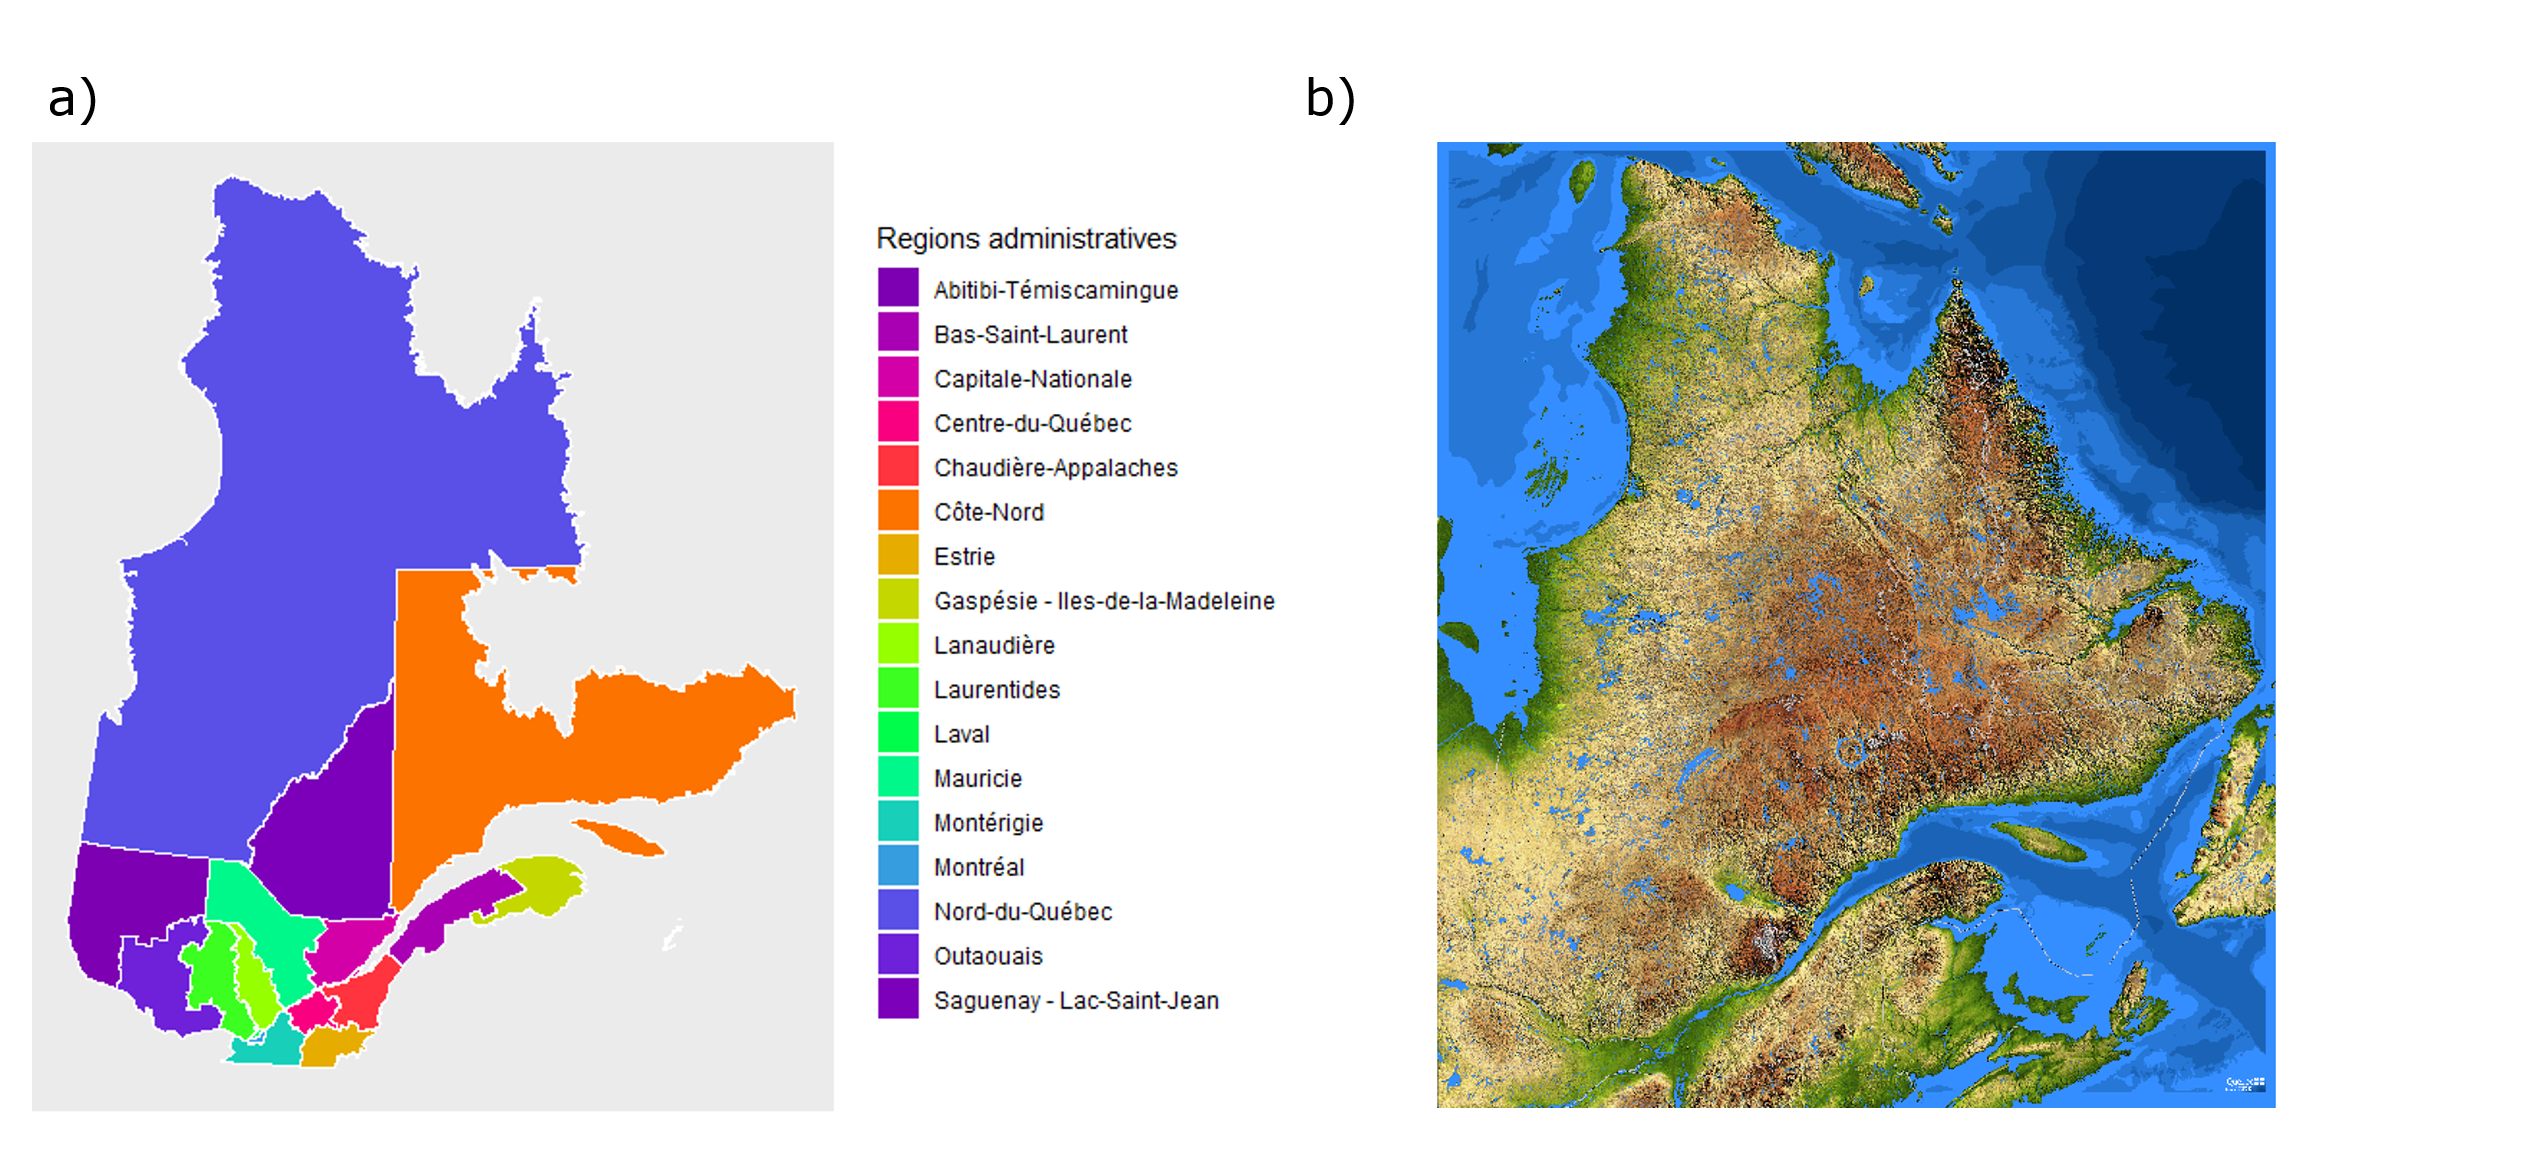
\includegraphics[width=1\linewidth]{Module2/images/2_vecto_vs_mat} \hfill{}

\caption{Exemples de données vectorielles et matricielles : a) La carte délimitant les régions administratives du Québec est formée à partir de données vectorielles; b) La carte topographique du Québec (source : [https://mern.gouv.qc.ca/repertoire-geographique/carte-relief-quebec/)](https://mern.gouv.qc.ca/repertoire-geographique/carte-relief-quebec/))}\label{fig:vectomat}
\end{figure}

Les entités spatiales (ou objets) sont habituellement représentés par ce qu'on appelle des données vectorielles (« vector data », en anglais), alors que les phénomènes continues sont habituellement représentés par des données matricielles (« raster data », en anglais). Ces deux modèles sont des façons bien différentes de percevoir et de représenter les phénomènes spatiaux. Nous les décrivons dans les deux sous-sections suivantes.

\hypertarget{les-donnuxe9es-vectorielles}{%
\subsubsection{Les données vectorielles}\label{les-donnuxe9es-vectorielles}}

\hypertarget{duxe9finition}{%
\paragraph{Définition}\label{duxe9finition}}
\addcontentsline{toc}{paragraph}{Définition}

Les données vectorielles sont utilisées pour représenter des entités spatiales dont les frontières sont explicites et qui possède une localisation précise et unique. Les données vectorielles sont définies par leur localisation géographique, leur géométrie, et un ou plusieurs attributs.

La \textbf{localisation géographique} désigne l'emplacement de l'entité selon un système de coordonnées géographiques ou un système de coordonnées projetées. Un système de coordonnées géographiques utilise un système en trois dimensions pour donner la position (x,y,z) ou longitude et latitude d'une entité spatiale sur la surface sphérique de la Terre. Un système de coordonnées projetées, donne la position d'une entité spatiale sur une surface plane à deux dimensions. Nous reviendrons sur les systèmes de coordonnées de référence à la section 2.1.3.

La \textbf{géométrie} d'une entité spatiale correspond à sa forme (« shape », en anglais). Il existe trois principaux types de géométrie, aussi appelées des classes : les points, les lignes, et les polygones (Tableau \ref{fig:geometriesimple}). Ces classes peuvent être combinées pour créer des géométries plus complexes; des multipoints, des multilignes, des multipolygones, etc.

\textbackslash begin\{figure\}

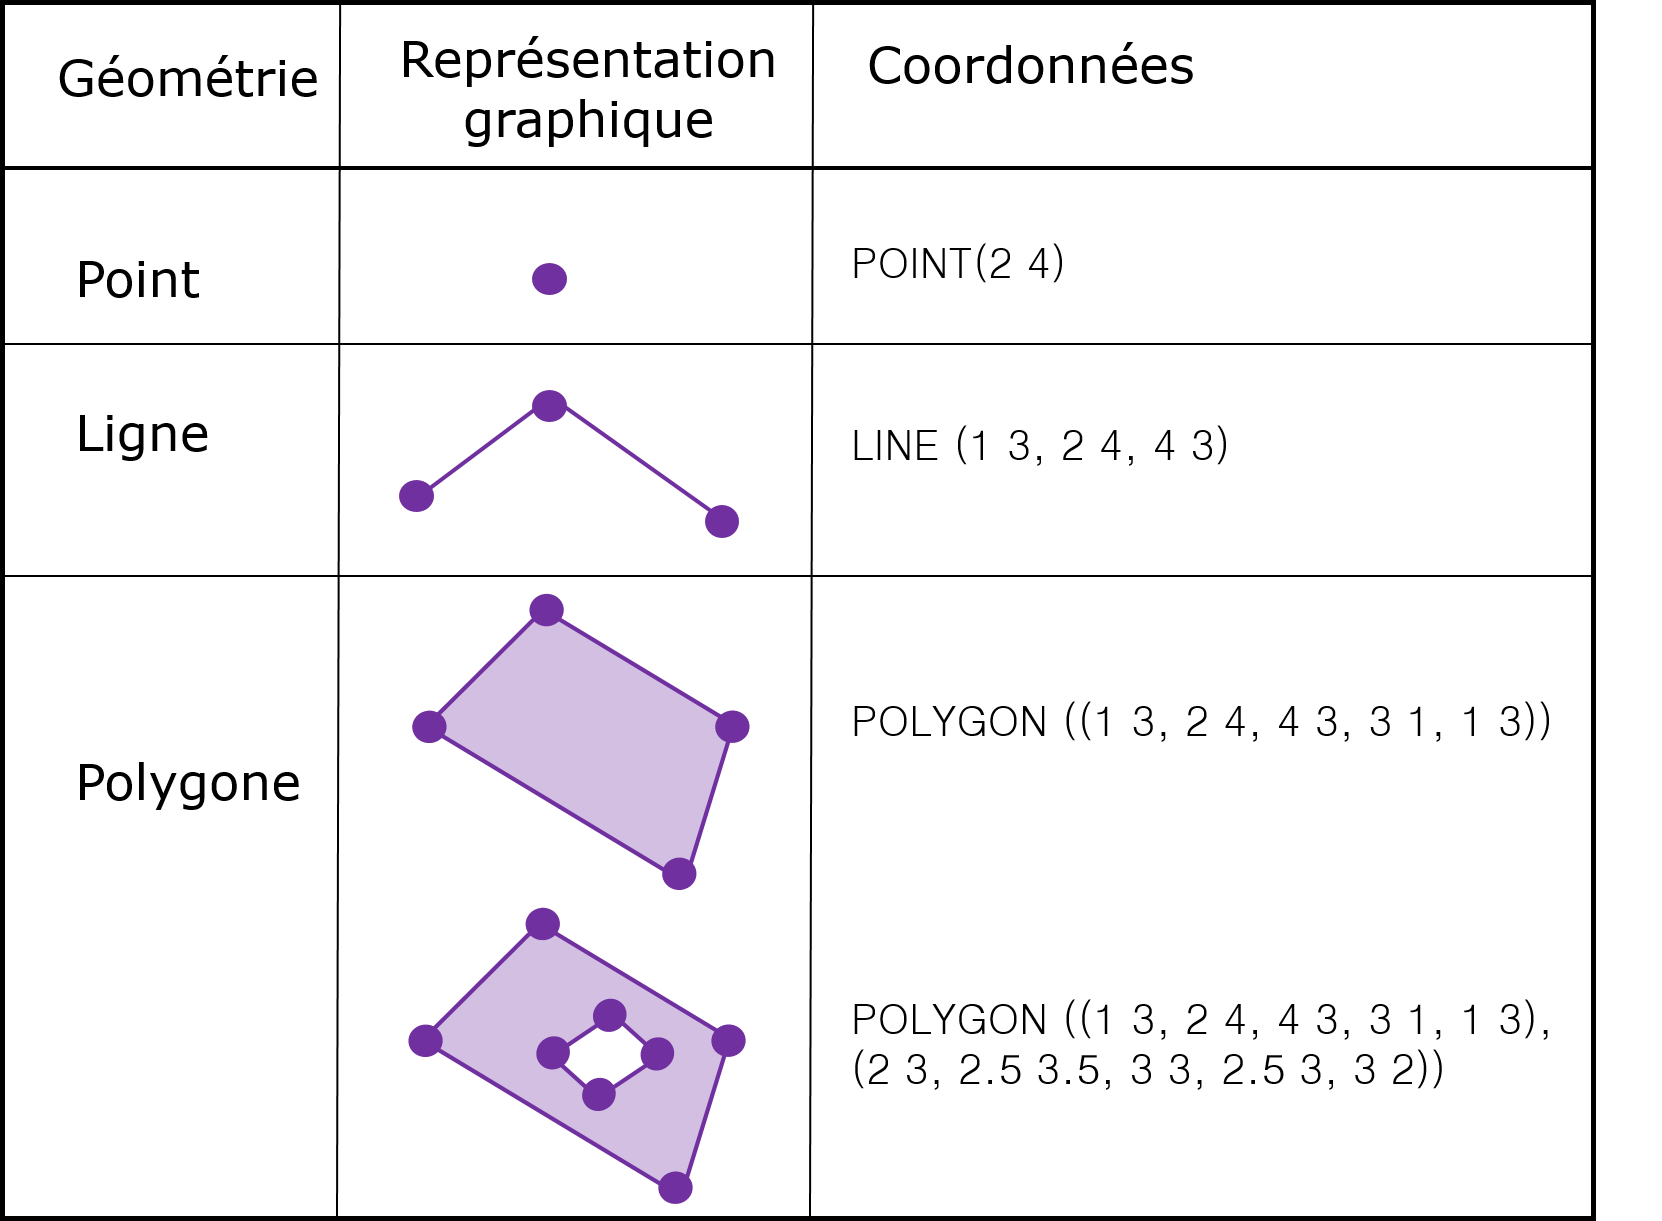
\includegraphics[width=0.8\linewidth]{Module2/images/2_geometriesimple} \hfill{}

\textbackslash caption\{Exemple de données vectorielles de géométrie simple. Remarquez que dans le cas d'un polygone, la première et la dernière coordonnées sont les mêmes. Tableau inspiré de Wikipedia (\url{https://en.wikipedia.org/wiki/Well-known_text_representation_of_geometry})\}\label{fig:geometriesimple}
\textbackslash end\{figure\}

Les données vectorielles comprennent également des variables additionnelles appelées des \textbf{attributs}. Les attributs sont toutes informations permettant de décrire une entité spatiale autres que sa localisation et sa géométrie.

\hypertarget{guxe9omuxe9trie-et-topologie}{%
\paragraph{Géométrie et topologie}\label{guxe9omuxe9trie-et-topologie}}
\addcontentsline{toc}{paragraph}{Géométrie et topologie}

Les \textbf{points} sont les données vectorielles les plus simples. Par exemple, un point pourrait représenter l'emplacement d'un restaurant dans une ville. Les attributs associés à ce point pourraient inclure les heures d'ouverture, sa spécialité culinaire, l'échelle de prix de son menu ou d'autres informations.

\begin{figure}

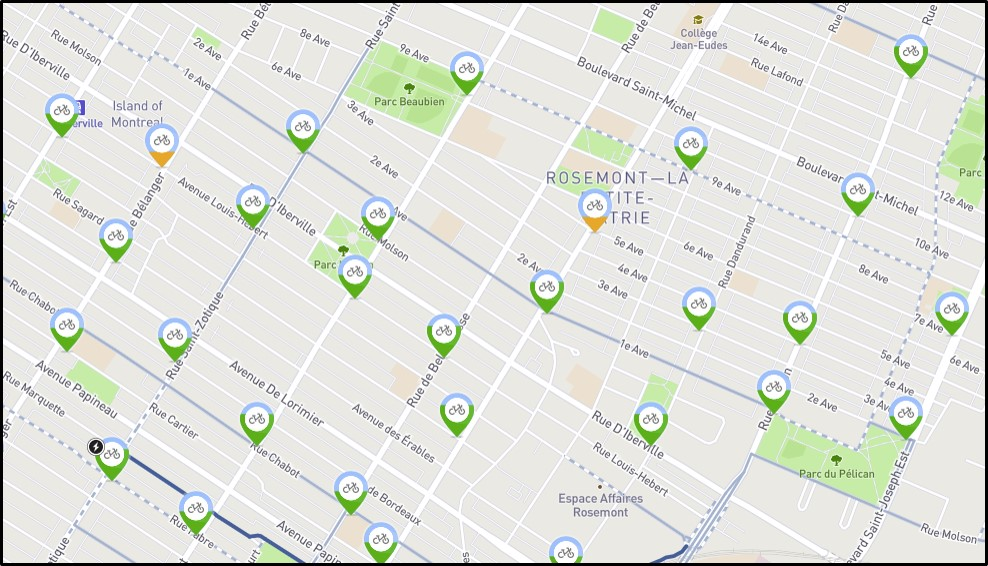
\includegraphics[width=0.6\linewidth]{Module2/images/2_multipoints} \hfill{}

\caption{L’emplacement des stations de vélo en libre partage, *Bixi*, dans un quartier de Montréal correspond à une géométrie multipoints. Source : https://secure.bixi.com/map/}\label{fig:multipoints}
\end{figure}

Il est aussi possible de combiner plusieurs points ensemble dans une structure multipoints définie par un attribut unique (Figure \ref{fig:multipoints}). Par exemple, l'ensemble des restaurants de cuisine vietnamienne dans une ville pourrait être considéré comme une géométrie unique.

La géométrie des \textbf{lignes} est plus complexe. Le terme ligne en analyse spatiale n'a pas la même définition que dans le langage usuel. Une ligne désigne un ensemble d'une seule ou de plusieurs polylignes (Figure \ref{fig:multilignes}). Une polyligne, quant à elle, désigne une séquence de segments de droite reliés entre eux. Ainsi, en analyse spatiale, une seule ligne pourrait représenter le fleuve Saint-Laurent et l'ensemble de ces affluents (rivière des Outaouais, rivière Saint-Maurice, le Fjord du Saguenay, etc.). D'autre part, il serait aussi possible de définir plusieurs lignes -- une pour chaque affluent, par exemple.

\begin{figure}

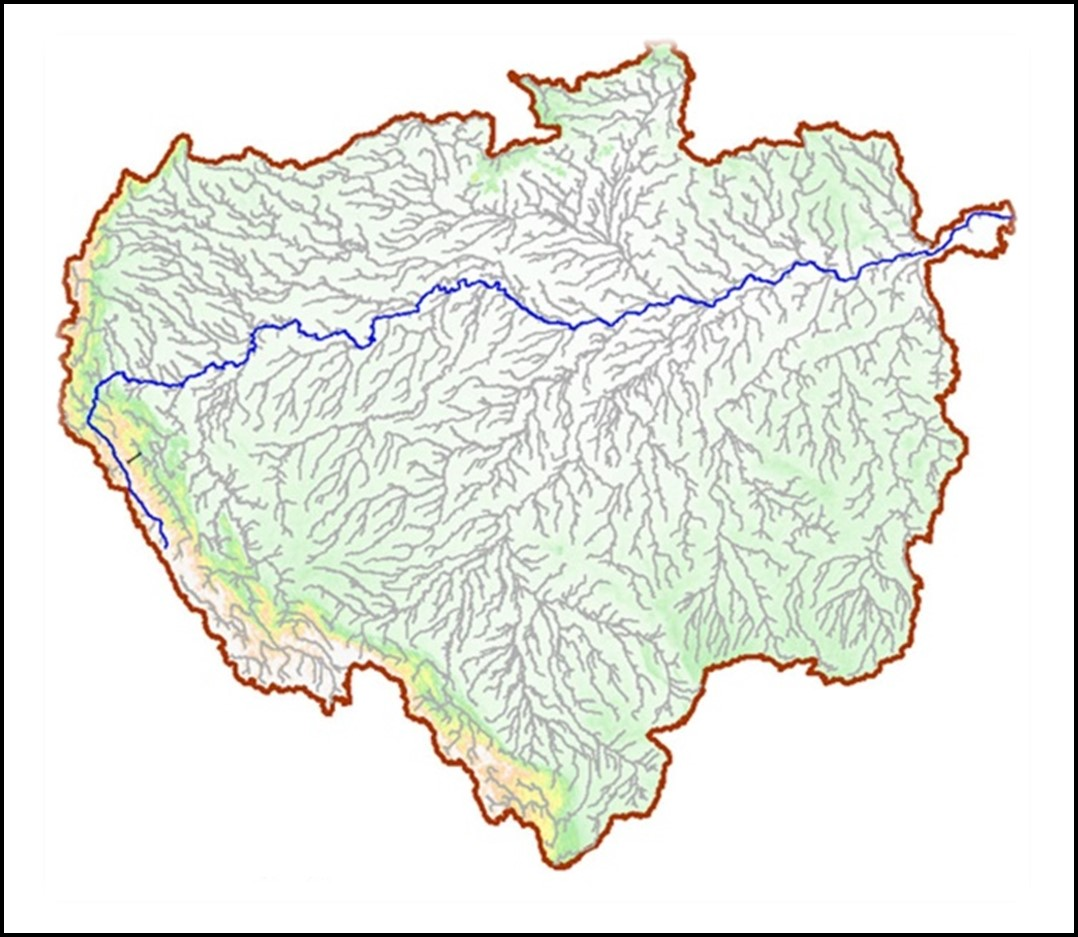
\includegraphics[width=0.6\linewidth]{Module2/images/2_multilignes} \hfill{}

\caption{Le réseau hydrologique du bassin de l’Amazone représente un exemple d’un ensemble de polylignes. Source : Wang et al. 2020.}\label{fig:multilignes}
\end{figure}

Une ligne est représentée par un ensemble ordonné de coordonnées. Les segments de droite peuvent être calculés ou dessinés sur une carte en connectant ensemble les points. Ainsi, la représentation d'une ligne est semblable à celle d'une structure multipoints. La différence notable est que l'ordre des points est important dans la représentation d'une ligne car il est nécessaire de savoir quels points sont connectés entre eux.

Un réseau -- par exemple un réseau routier ou un réseau hydrographique -- est une ligne de géométrie particulière comprenant des informations additionnelles comme le débit, la connectivité ou la distance.

Un \textbf{polygone} désigne un ensemble de polylignes fermées. La géométrie d'un polygone est très semblable à celle des lignes à l'exception que la dernière paire de coordonnées doit coïncider avec la première paire afin de « fermer » le polygone.

Une particularité des polygones est qu'ils peuvent comprendre des trous. C'est-à-dire qu'un polygone peut être entièrement compris à l'intérieur d'un polygone de plus grande superficie. Ceci est le cas d'une île au sein d'un lac, par exemple. Le polygone formant un îlot permet d'éliminer une partie du polygone qui l'englobe. De plus, alors que l'auto-intersection est permise pour une ligne (c'est-à-dire qu'elle peut se croiser sur elle-même), cette propriété n'est pas valide pour un polygone.

Finalement, plusieurs polygones peuvent être considérés comme formant une géométrie unique ((Figure \ref{fig:multipolygones})). Par exemple, l'Indonésie est constituée de plusieurs îles. Chaque île peut être représentée par son propre polygone, ou encore l'ensemble des îles peut être représenté par un seul polygone (ou multi-polygones) désignant le pays en entier.

\begin{figure}

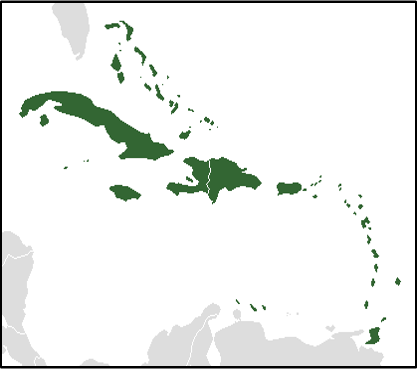
\includegraphics[width=0.5\linewidth]{Module2/images/2_multipolygones} \hfill{}

\caption{Les Antilles peuvent être représentées par plusieurs polygones distincts pour chaque île, ou par un seul multipolygone. Source : https://fr.wikipedia.org/wiki/Antilles}\label{fig:multipolygones}
\end{figure}

Le modèle vectoriel est très efficace pour représenter la \textbf{topologie}. La topologie est une description des relations spatiales qu'ont les entités spatiales entre elles. Par exemple, une analyse de données vectorielles permettra de déterminer précisément si une entité spatiale est adjacente à une autre, si elle y est incluse, ou si elle s'intersecte (Figure \ref{fig:relationsspatiales}).

\begin{figure}

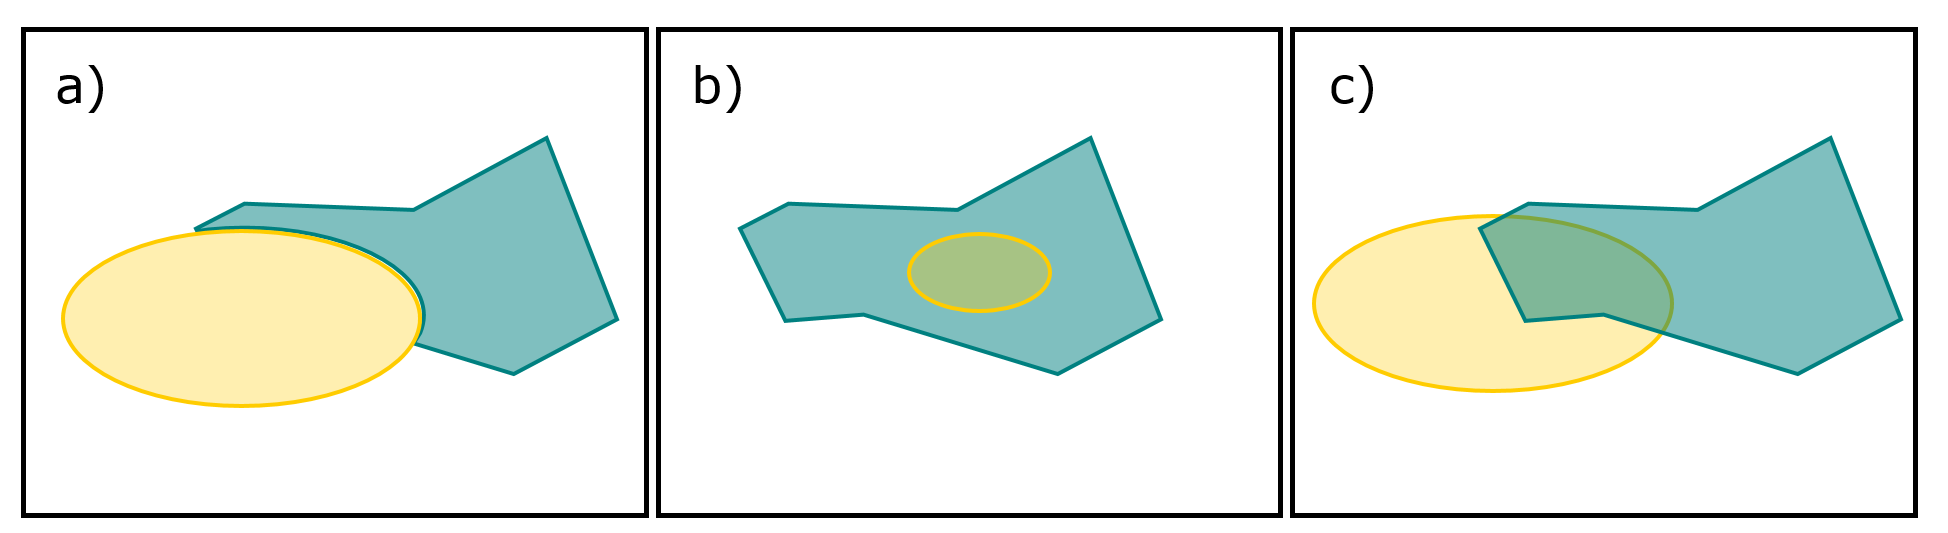
\includegraphics[width=1\linewidth]{Module2/images/2_relationsspatiales} \hfill{}

\caption{Exemples de relations spatiales entre deux entités spatiales : a) adjacence, b) inclusion, et c) intersection.}\label{fig:relationsspatiales}
\end{figure}

\hypertarget{format-de-donnuxe9es-vectorielles}{%
\paragraph{Format de données vectorielles}\label{format-de-donnuxe9es-vectorielles}}
\addcontentsline{toc}{paragraph}{Format de données vectorielles}

Les données vectorielles peuvent être stockées dans une grande variété de formats différents. Ces formats ont évolué et continuent d'évoluer en fonction des besoins et des avancées technologiques. Plusieurs formats ont été développés pour être utilisés avec des logiciels commerciaux mais peuvent être lus et parfois édités par d'autres logiciels.

Peu importe leur format, les données vectorielles sont toujours organisées selon une \emph{base de données relationnelle}. Un identifiant désigne chaque objet spatial et l'associe à une géométrie et à un ou plusieurs attributs (Tableau \ref{fig:baserelationnelle}).

\begin{figure}

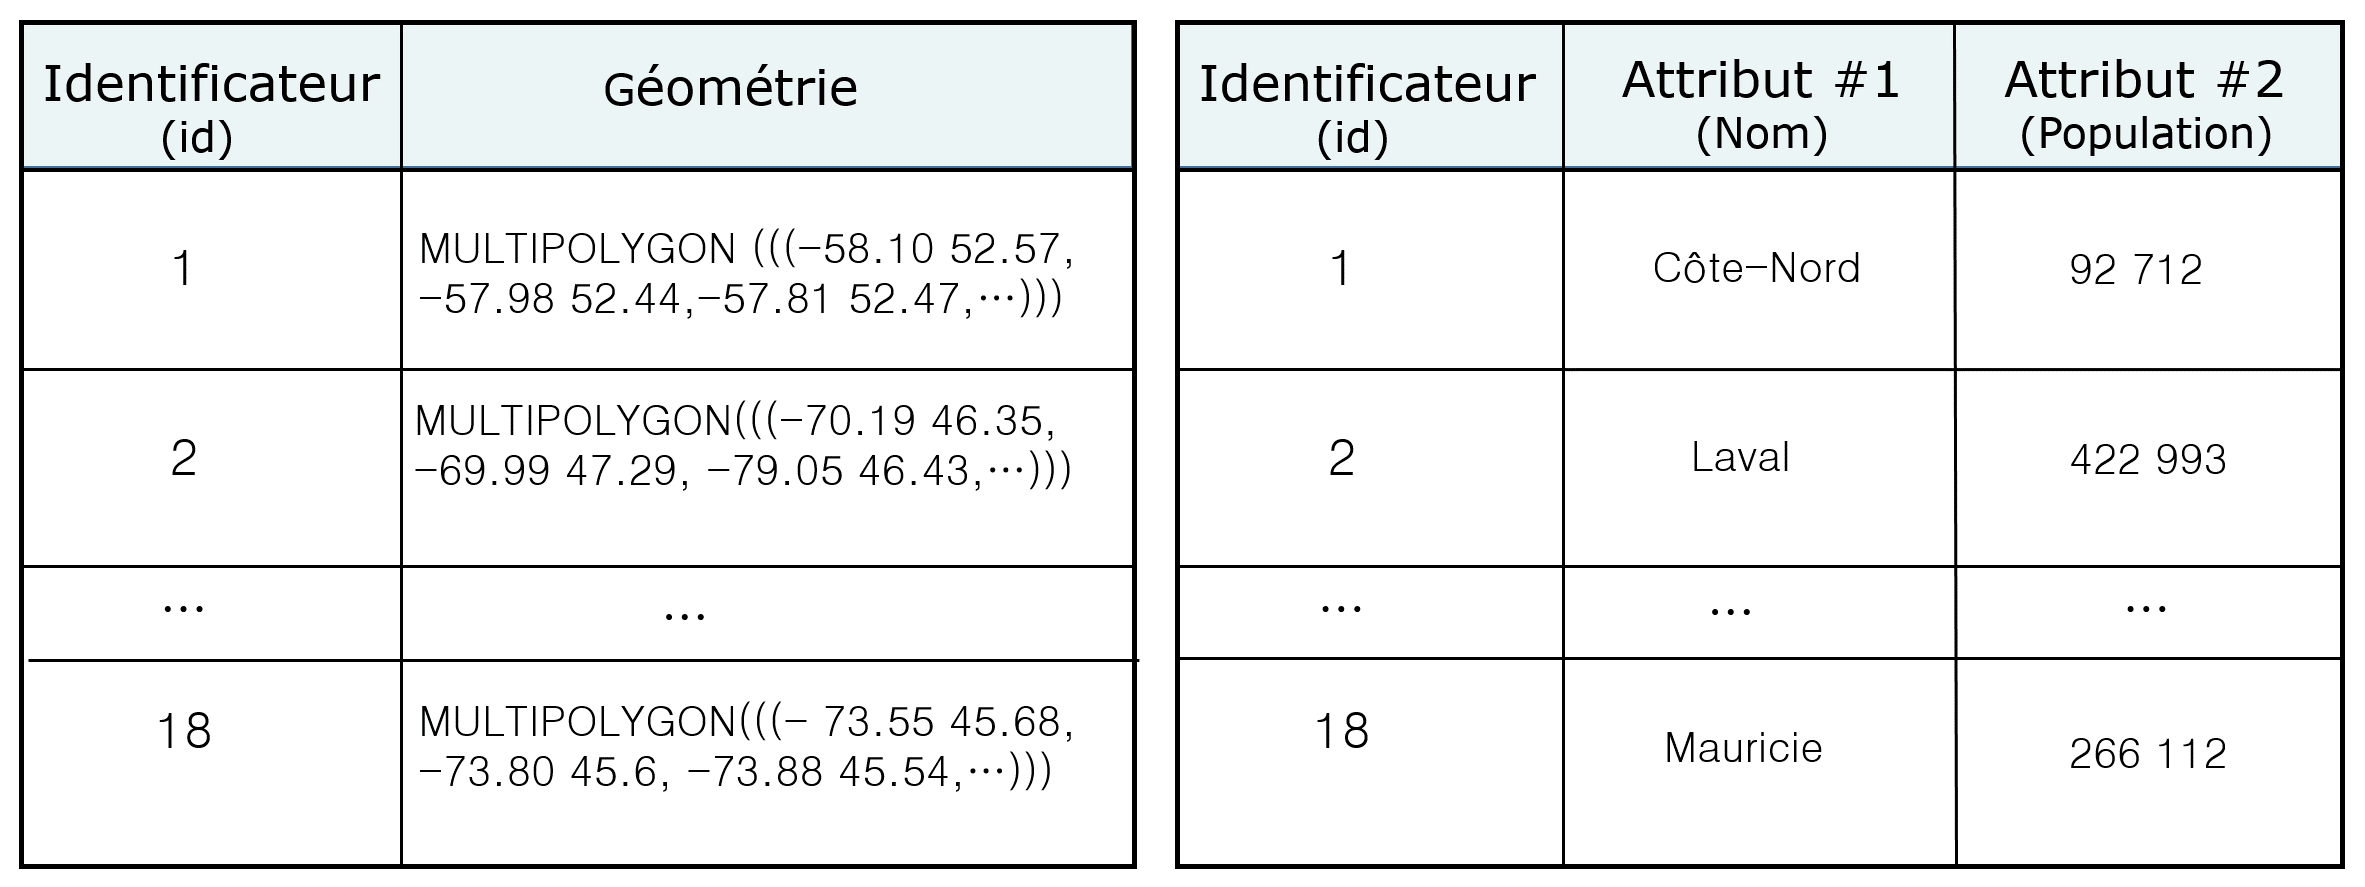
\includegraphics[width=1\linewidth]{Module2/images/2_baserelationnelle} \hfill{}

\caption{Exemple d’une base de données relationnelle pour la carte des régions administratives du Québec (Figure ref(fig:vectomat)a). Chaque objet vectoriel dans la carte correspond à une ligne dans la base de données où figurent les attributs qui lui sont associés}\label{fig:baserelationnelle}
\end{figure}

Voici une liste non-exhaustive de formats de données vectorielles.

\begin{quote}
SHAPEFILE (.SHP, .DBF, .PRJ, .SHX)
\end{quote}

Le \emph{shapefile} est un format propriétaire d'ESRI créé pour les logiciels ArcView et ArcGIS. En français, on le nomme aussi un fichier de forme. À ce jour, il est le format le plus couramment utilisé pour les données vectorielles. Il est devenu un standard tant pour les plateformes commerciales qu'opensource.

Un \emph{shapefile} comprend entre quatre types de fichiers qui contiennent des informations différentes et toutes essentielles à sa représentation.

\begin{itemize}
\tightlist
\item
  .shp : contient les données spatiales
\item
  .dbf : contient les données d'attributs
\item
  .prj : contient l'information sur la projection des données
\item
  .shx : fichier d'index
\end{itemize}

Le fichier d'index sert à lier entre elles les informations contenues dans les autres fichiers. Il existe parfois d'autres types de fichier d'index (.sbx, .sbn). Pour visualiser un \emph{shapefile}, il est nécessaire d'avoir tous les fichiers associés (et pas seulement le fichier .shp). Le fichier .prj peut être absent. En son absence, le shapefile peut être lu mais les données ne seront pas projetées adéquatement. Nous reviendrons sur le concept de projection plus tard dans ce module.

\begin{quote}
GEODATABASE
\end{quote}

La géodatabase est le nouveau format propriétaire d'ESRI conçu pour ArcGIS. Il est de plus en plus adopté car il présente de nombreux avantages par rapport au \emph{shapefile}. Une géodatabase est une façon de rassembler et d'organiser des données propres à un sujet ou à un projet dans une unique base de données. Elle peut contenir des données géographiques dans une large gamme de fichiers et de formats (Figure \ref{fig:geodatabase}).

\begin{figure}

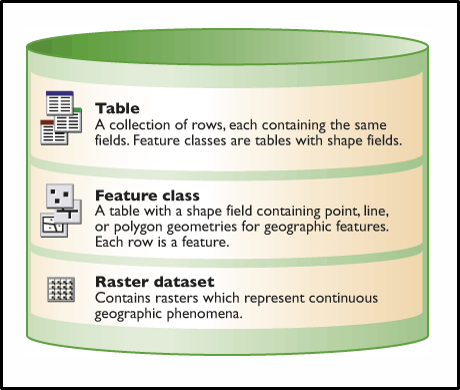
\includegraphics[width=0.5\linewidth]{Module2/images/2_geodatabase} \hfill{}

\caption{Illustration d’une géodatabase telle que représentée sur le site web d’ArcGIS. Image récupérée à : https://desktop.arcgis.com/fr/arcmap/10.3/manage-data/geodatabases/a-quick-tour-of-the-geodatabase.htm}\label{fig:geodatabase}
\end{figure}

Par exemple, un projet sur le réseau de transport d'électricité au Québec pourrait nécessiter l'utilisation de plusieurs \emph{shapefiles} (position des centrales, position des pylônes, parcours des câbles, etc.) et aussi plusieurs données matricielles (topographie, végétation, etc.). Ainsi, il s'avère beaucoup plus efficace d'avoir l'ensemble de ces données au sein d'une même base.

De plus, une géodatabase peut être utilisée par de multiples utilisateurs, ce qui est fort utile pour assurer le partage efficace, la mise à jour, et la cohérence des données géographiques au sein de grandes organisations, comme des entreprises ou des ministères.

Malheureusement, bien que les géodatabases peuvent être lues avec \texttt{R}, elles peuvent seulement être modifiées dans ArcGIS.

\begin{quote}
GEOGRAPHIC JAVASCRIPT OBJECT NOTATION (.GEOJSON, .JSON)
\end{quote}

Le format geoJSON est un format standard ouvert très utilisé en cartographie web. geoJSON est une extension du format JSON pour les données géographiques. Un fichier geoJSON contient les coordonnées des données géospatiales ainsi que d'autres informations sur les attributs. Un seul fichier est nécessaire pour stocker l'ensemble de l'information.

\begin{quote}
GOOGLE KEYHOLE MARKUP LANGUAGE (.KML, .KMZ)
\end{quote}

Ce format est basé sur le langage XML et est optimisé pour les navigateurs de cartographie web comme Google Maps et Google Earth. KMZ est une version compressée d'un fichier KML (KML-Zipped).

\begin{quote}
COVERAGE
\end{quote}

COVERAGE est le format propriétaire d'ESRI, développé pour le logiciel ArcInfo, qui a précédé le format \emph{shapefile}. C'est une autre façon de stockée les données vectorielles qui nécessite plusieurs fichiers. Bien que ce format ne soit plus utilisé lorsque de nouvelles données vectorielles sont conçues, vous pourriez être amenés à rencontrer ce format si vous devez travailler avec des données qui précédent 1990.

\begin{quote}
ARCINFO INTERCHANGE FILE (.EOO)
\end{quote}

C'est le format utilisé pour importer ou exporter des données d'ArcInfo. Il fonctionne comme un fichier zip et permet de partager facilement en un seul fichier les multiples fichiers et dossiers associés au format Coverage. Il permet aussi de transférer des données matricielles de format GRID.

\begin{quote}
MAPINFO INTERCHANGE FILE (.MID, .MIF)
\end{quote}

C'est le format propriétaire de MapInfo, le compétiteur d'Esri. Le format \emph{shapefile} a supplanté le format interchange qui est de moins en moins utilisé. Le fichier MIF contient la localisation géographique et la topologie, et le fichier MID contient les attributs.

\begin{quote}
WEB MAP SERVICE (WMS)
\end{quote}

N'est pas un format de données mais plutôt un protocole de communication qui permet de visualiser des données spatiales qui sont logées sur un serveur. Les organisations gouvernementales ont souvent recours à cette méthode de partage de l'information spatiale car elle permet de s'assurer que les données diffusées sont toujours à jour. L'utilisateur peut jouer avec les paramètres de visualisation mais ne peut pas importer et modifier les données. Notez que ce protocole est utilisé à la fois pour les données vectorielles et les données matricielles.

\hypertarget{les-donnuxe9es-matricielles}{%
\subsubsection{Les données matricielles}\label{les-donnuxe9es-matricielles}}

\hypertarget{duxe9finition-1}{%
\paragraph{Définition}\label{duxe9finition-1}}
\addcontentsline{toc}{paragraph}{Définition}

Les données matricielles représentent la surface terrestre par une grille régulière, communément appelé un raster, formée de rectangles de même forme et de même dimension appelés cellules ou pixels (Figure \ref{fig:raster}). À chaque cellule de la matrice est associée une valeur numérique (ou une valeur manquante) associée à un attribut d'intérêt. On appelle couche (« layer » en anglais) l'information recueillie dans la matrice.

La valeur d'une cellule peut être continue (p.~ex. l'élévation - voir Figure \ref{fig:vectomat}b) ou catégorique (p.~ex. le zonage attribué à différents secteurs d'une ville tel que résidentiel, commercial ou industriel). Normalement, la valeur d'une cellule représente la valeur moyenne (ou la valeur prédominante) pour la superficie qu'elle couvre. Cependant, les valeurs sont parfois estimées pour le centre de la cellule.

\begin{figure}

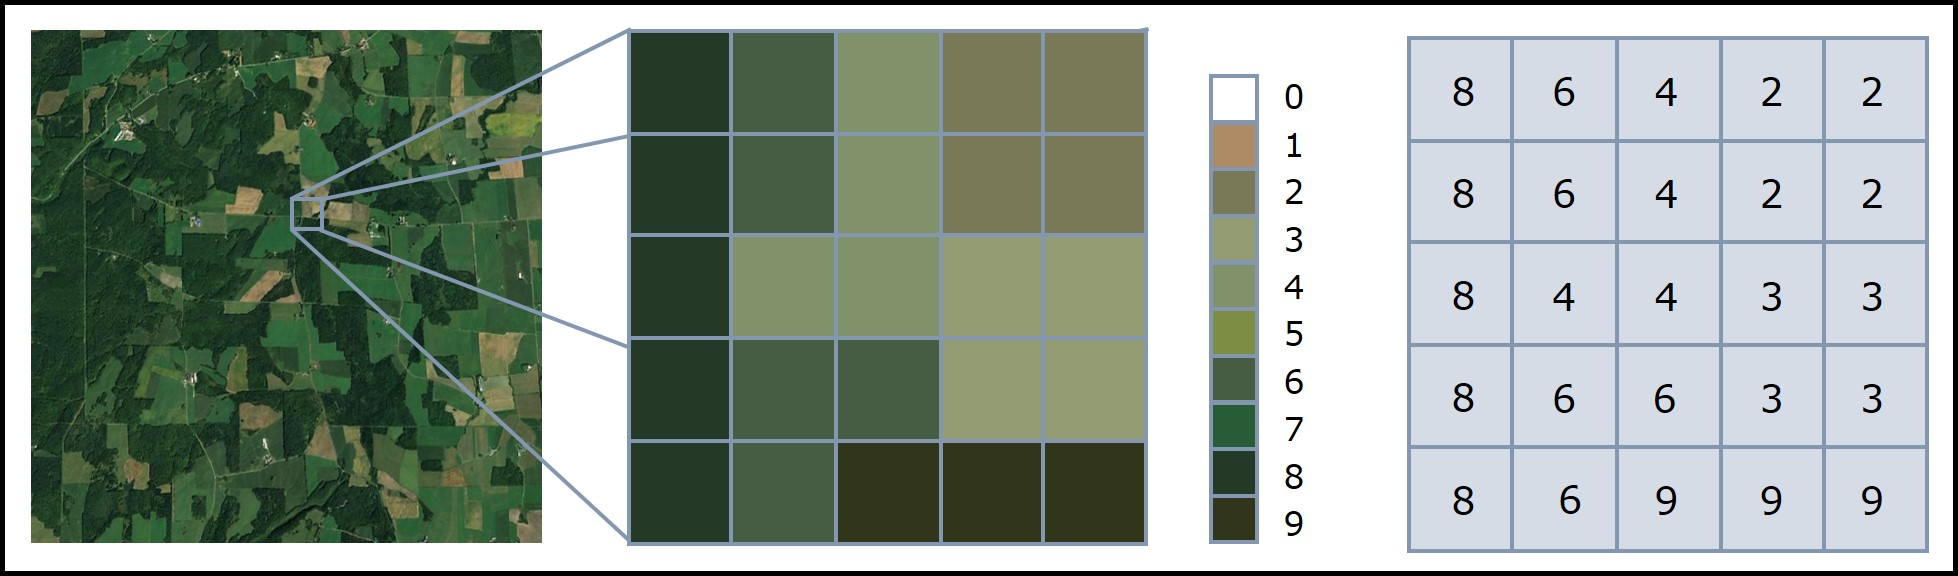
\includegraphics[width=1\linewidth]{Module2/images/2_raster} \hfill{}

\caption{Exemple de données matricielles associées à des classes de végétation obtenues à partir d’une image satellitaire. Figure inspirée de NEON neonscience.org/resources/series/introduction-working-raster-data-r}\label{fig:raster}
\end{figure}

On peut utiliser une base de données relationnelle pour lier la valeur d'un pixel à l'attribut qu'il décrit (Figure \ref{fig:rastertable}). Contrairement aux données vectorielles où les polygones peuvent être associés à plusieurs attributs, une couche de données matricielles peut représenter un seul attribut.

\begin{figure}

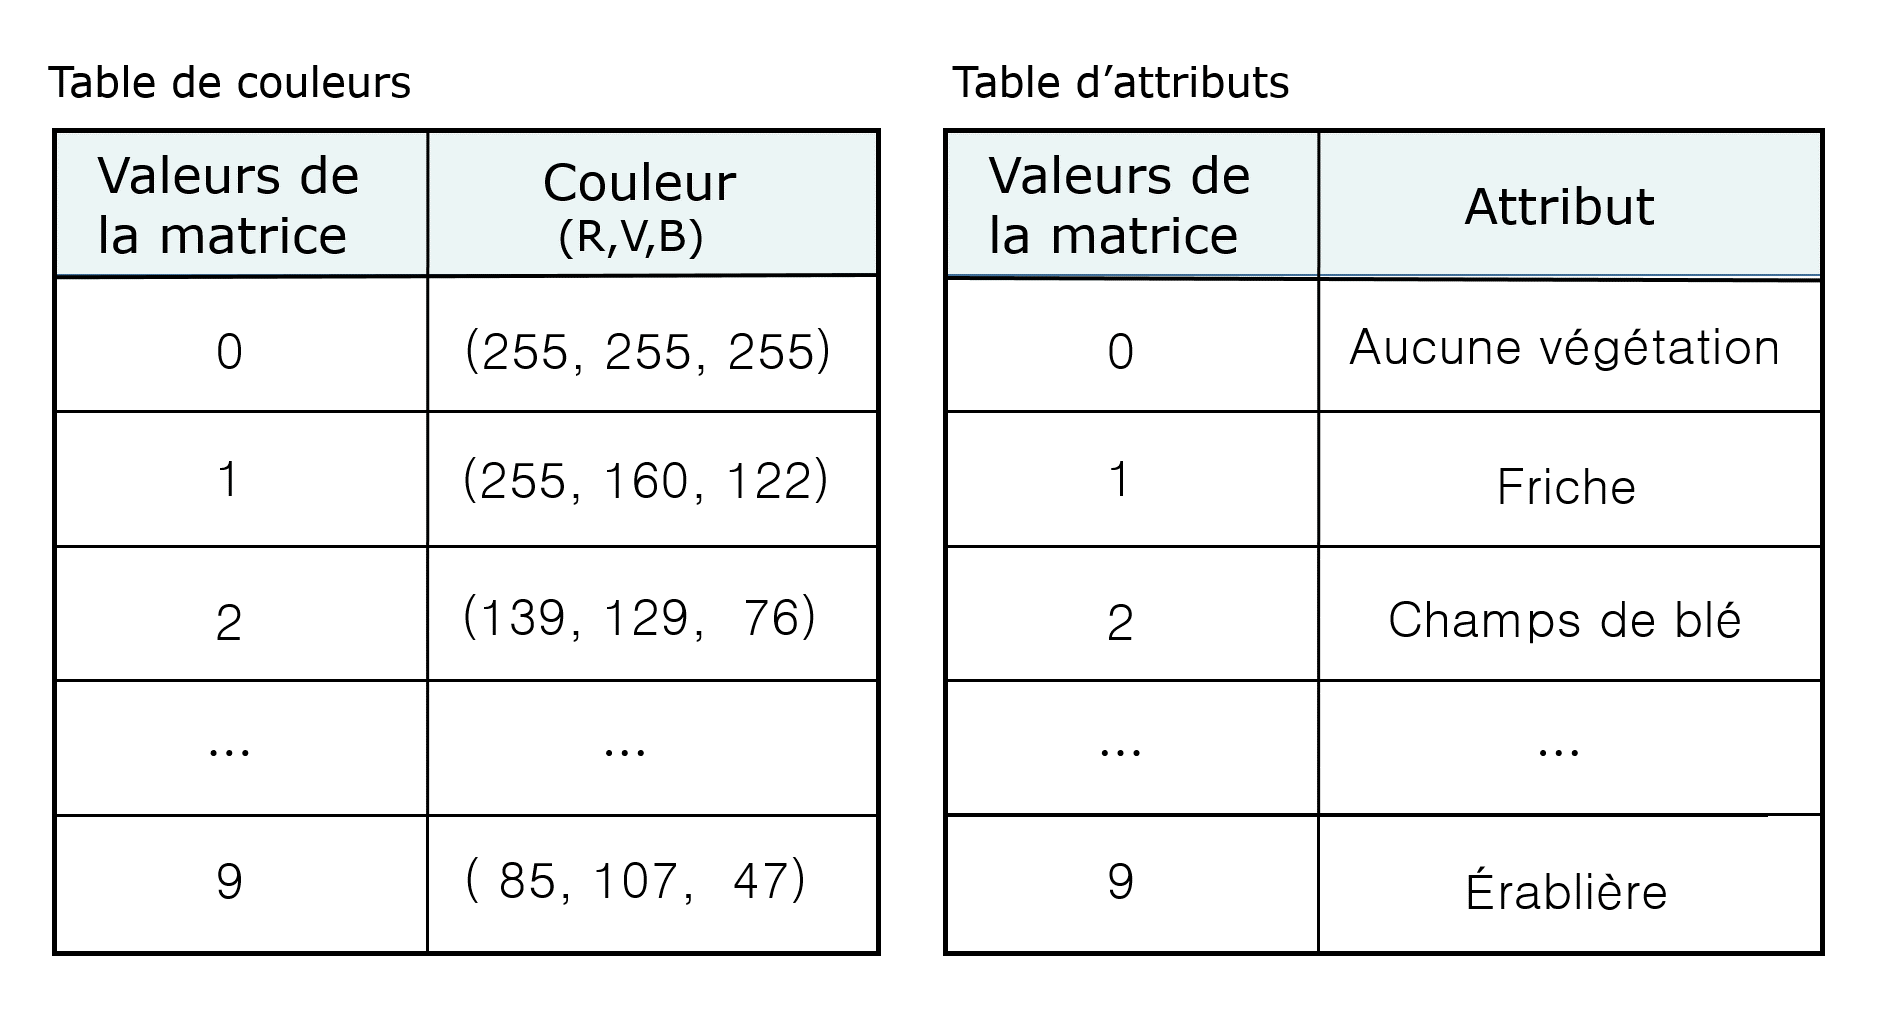
\includegraphics[width=0.8\linewidth]{Module2/images/2_raster_table} \hfill{}

\caption{Exemple de table relationnelle pour les données vectorielles de la Figure ref(fig:raster). Une valeur numérique est associée à chaque couleur de l’image ainsi qu’à un attribut, ici le type de végétation}\label{fig:rastertable}
\end{figure}

Dans leur format le plus simple, les données matricielles prennent la forme d'une image digitale. Cependant, pour associer les données matricielles à une location particulière sur la surface de la Terre, des informations spatiales doivent être ajoutées. Ainsi, un fichier de données matricielles géospatiales débute toujours par une section, appelée le «header» en anglais, qui procure la localisation.

La localisation pour des données matricielles est définie par \textbf{l'étendue spatiale} (« extent » en anglais) couverte par la matrice, la \textbf{dimension} des cellules, le \textbf{nombre de rangées et de colonnes} qui divisent la superficie (respectivement « rows » et « columns » en anglais), et le \textbf{système de coordonnées géographiques ou projetées}. La dimension des cellules correspond à la résolution spatiale et peut être calculée à partir de l'étendue et du nombre de rangées et de colonnes.

\hypertarget{ruxe9solution-et-guxe9omuxe9trie}{%
\paragraph{Résolution et géométrie}\label{ruxe9solution-et-guxe9omuxe9trie}}
\addcontentsline{toc}{paragraph}{Résolution et géométrie}

La \textbf{résolution} définie la précision avec laquelle nous pouvons discerner les objets dans l'espace. Une grande résolution correspond à une matrice de données dont les cellules ont une petite taille (Figure \ref{fig:resolution}). En conséquence, une telle matrice est plus lente à visualiser et à manipuler, et requière un fichier plus volumineux. En contrepartie, une couche de données matricielles de faible résolution possède des cellules de plus grande taille, se visualise et se manipule plus rapidement, et est contenue dans un fichier moins volumineux.

\begin{figure}

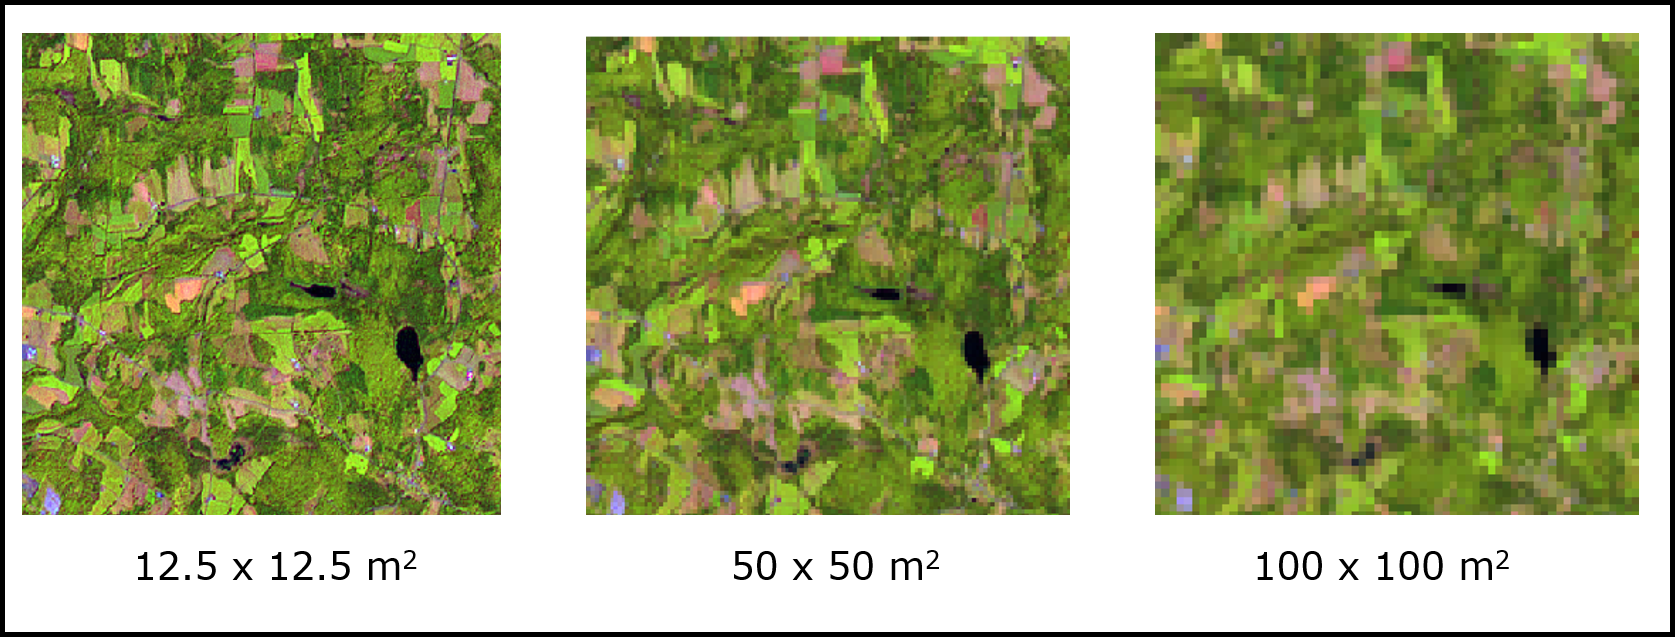
\includegraphics[width=1\linewidth]{Module2/images/2_resolution} \hfill{}

\caption{Exemple du concept de résolution: plus la résolution est grande, plus la taille des cellules est petite. Dans cette figure, la résolution diminue de droite à gauche, et la taille des cellules augmente. Source de données: https://mern.gouv.qc.ca/nos-publications/spatiocarte-quebec/}\label{fig:resolution}
\end{figure}

Contrairement aux données vectorielles, la géométrie des données matricielles n'est pas définie explicitement par un ensemble de coordonnées. La géométrie peut être déduite en observant les démarcations se produisant aux limites des ensembles de cellules de même valeur. Cependant ces démarcations ne correspondent pas nécessairement aux frontières des entités sur le terrain (Figure \ref{fig:boundary}).

\begin{figure}

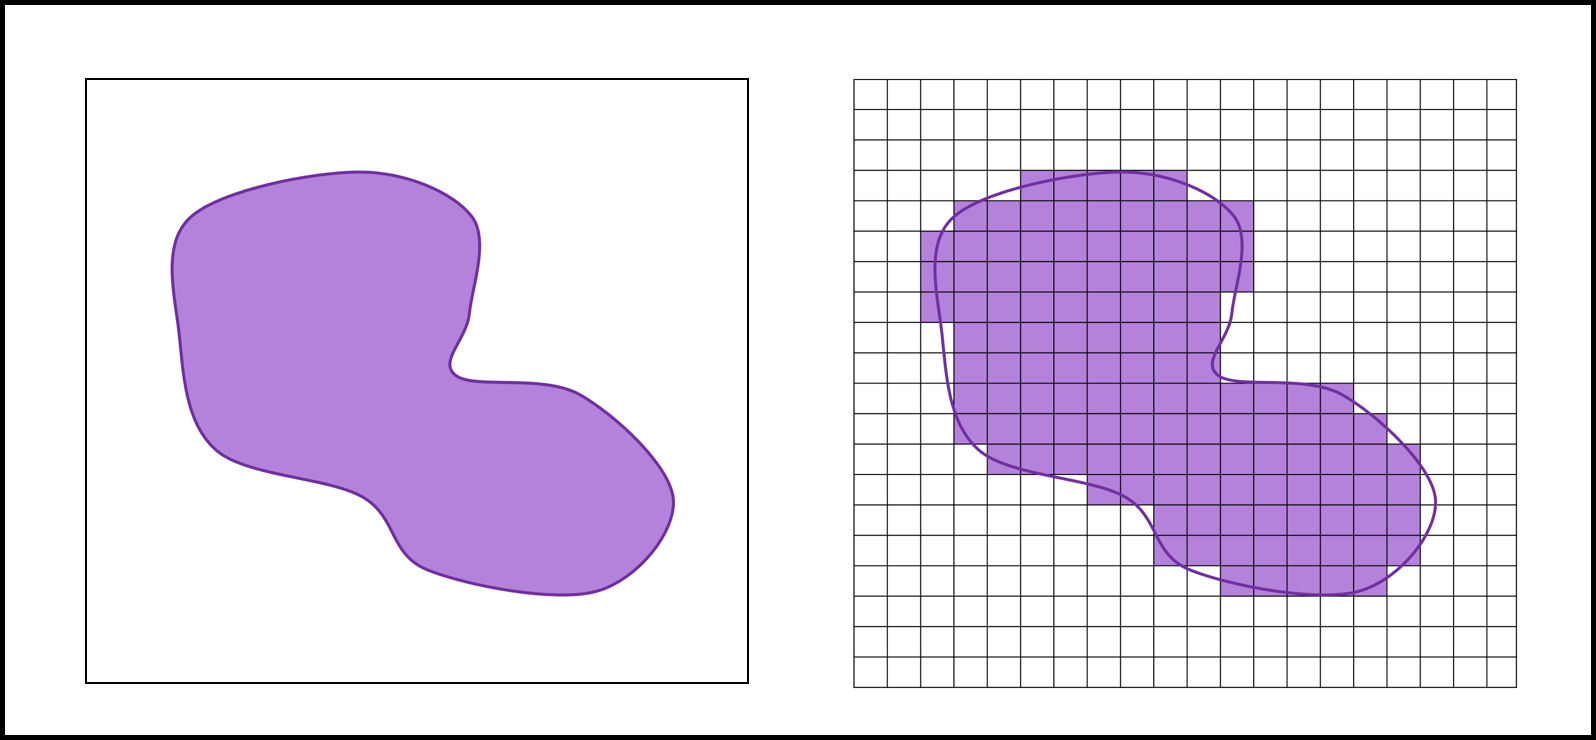
\includegraphics[width=0.8\linewidth]{Module2/images/2_raster_boundary} \hfill{}

\caption{La géométrie des objets spatiaux matriciels. Les frontières d’une entité spatiale définie avec des données matricielles (droite) ne correspondent pas nécessairement aux frontières réelles (gauche)}\label{fig:boundary}
\end{figure}

Ainsi, lorsque nous représentons des objets spatiaux aux frontières bien définies, l'utilisation de données vectorielles plutôt que matricielles s'avère plus précise et plus efficace.

Par ailleurs, la représentation de phénomènes continus avec des données vectorielles, nécessiterait de définir un grand nombre de petit polygones et d'enregistrer les coordonnées de chacun d'eux. Dans la majorité des cas, une telle représentation augmenterait dramatiquement le temps de traitement des données.

\hypertarget{donnuxe9es-matricielles-uxe0-bande-unique-et-multi-bandes}{%
\paragraph{Données matricielles à bande unique et multi-bandes}\label{donnuxe9es-matricielles-uxe0-bande-unique-et-multi-bandes}}
\addcontentsline{toc}{paragraph}{Données matricielles à bande unique et multi-bandes}

Un \emph{raster} peut contenir une couche ou plusieurs couches de données. Par exemple, un fichier de données matricielles d'élévation comprendra une seule couche de données, soit l'élévation à chaque cellule. Par exemple la carte topographique du Québec (Figure \ref{fig:vectomat}b) est un exemple de raster à une seule couche.

Un raster à une seule couche peut aussi représenter des images en noir et blanc en utilisant un codage binaire pour exprimer différentes teintes de gris. Un codage sur 1 bit exprimera 21 (2) teintes de gris {[}0,1{]}, un codage sur 4 bit exprimera 24 (16) teintes de gris {[}0,1,2,\ldots,15{]}, et un codage sur 16 bits exprimera 216 (65536) teintes de gris {[}0,1,2,\ldots, 65535{]} (Figure \ref{fig:binaire}).

\begin{figure}

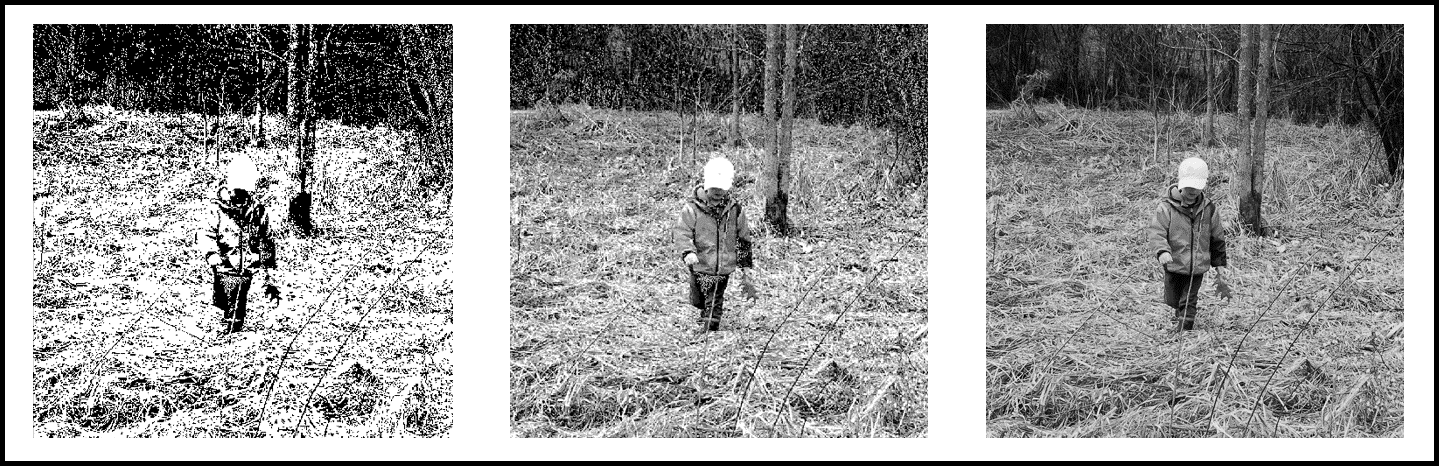
\includegraphics[width=1\linewidth]{Module2/images/2_binaire} \hfill{}

\caption{Exemple de codage binaire pour les *raster* à une couche: Images en blanc et noir utilisant différentes teintes de gris : 2 teintes (gauche), 8 teintes (centre) et 256 teintes (droite).}\label{fig:binaire}
\end{figure}

D'autres rasters peuvent contenir plusieurs couches, appelées aussi des bandes (ou canaux). Par exemple, les images de couleurs contiennent souvent trois bandes: une bande de rouge, une bande de vert et une bande de bleu. C'est ce qu'on nomme le format RGB (pour « red », « green », et « blue »). Ces bandes font références à des sections du spectre électromagnétique captées lors de la prise de l'image (Figure \ref{fig:electro}).

\begin{figure}

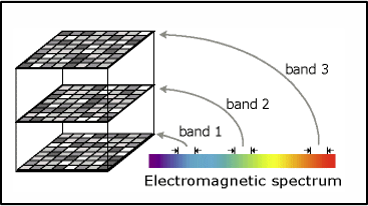
\includegraphics[width=0.5\linewidth]{Module2/images/2_electromagnetic_spectrum} \hfill{}

\caption{*Raster* multibande. Les bandes blues, vertes et rouges correspondent à des sections du spectre électromagnétique. Image récupérée à https://desktop.arcgis.com/en/arcmap/10.3/manage-data/raster-and-images/raster-bands.htm.}\label{fig:electro}
\end{figure}

En combinant ces bandes, on peut recréer l'image (Figure \ref{fig:3bands}). Attention : chaque bande doit posséder les mêmes informations spatiales pour être superposée aux autres.

\begin{figure}

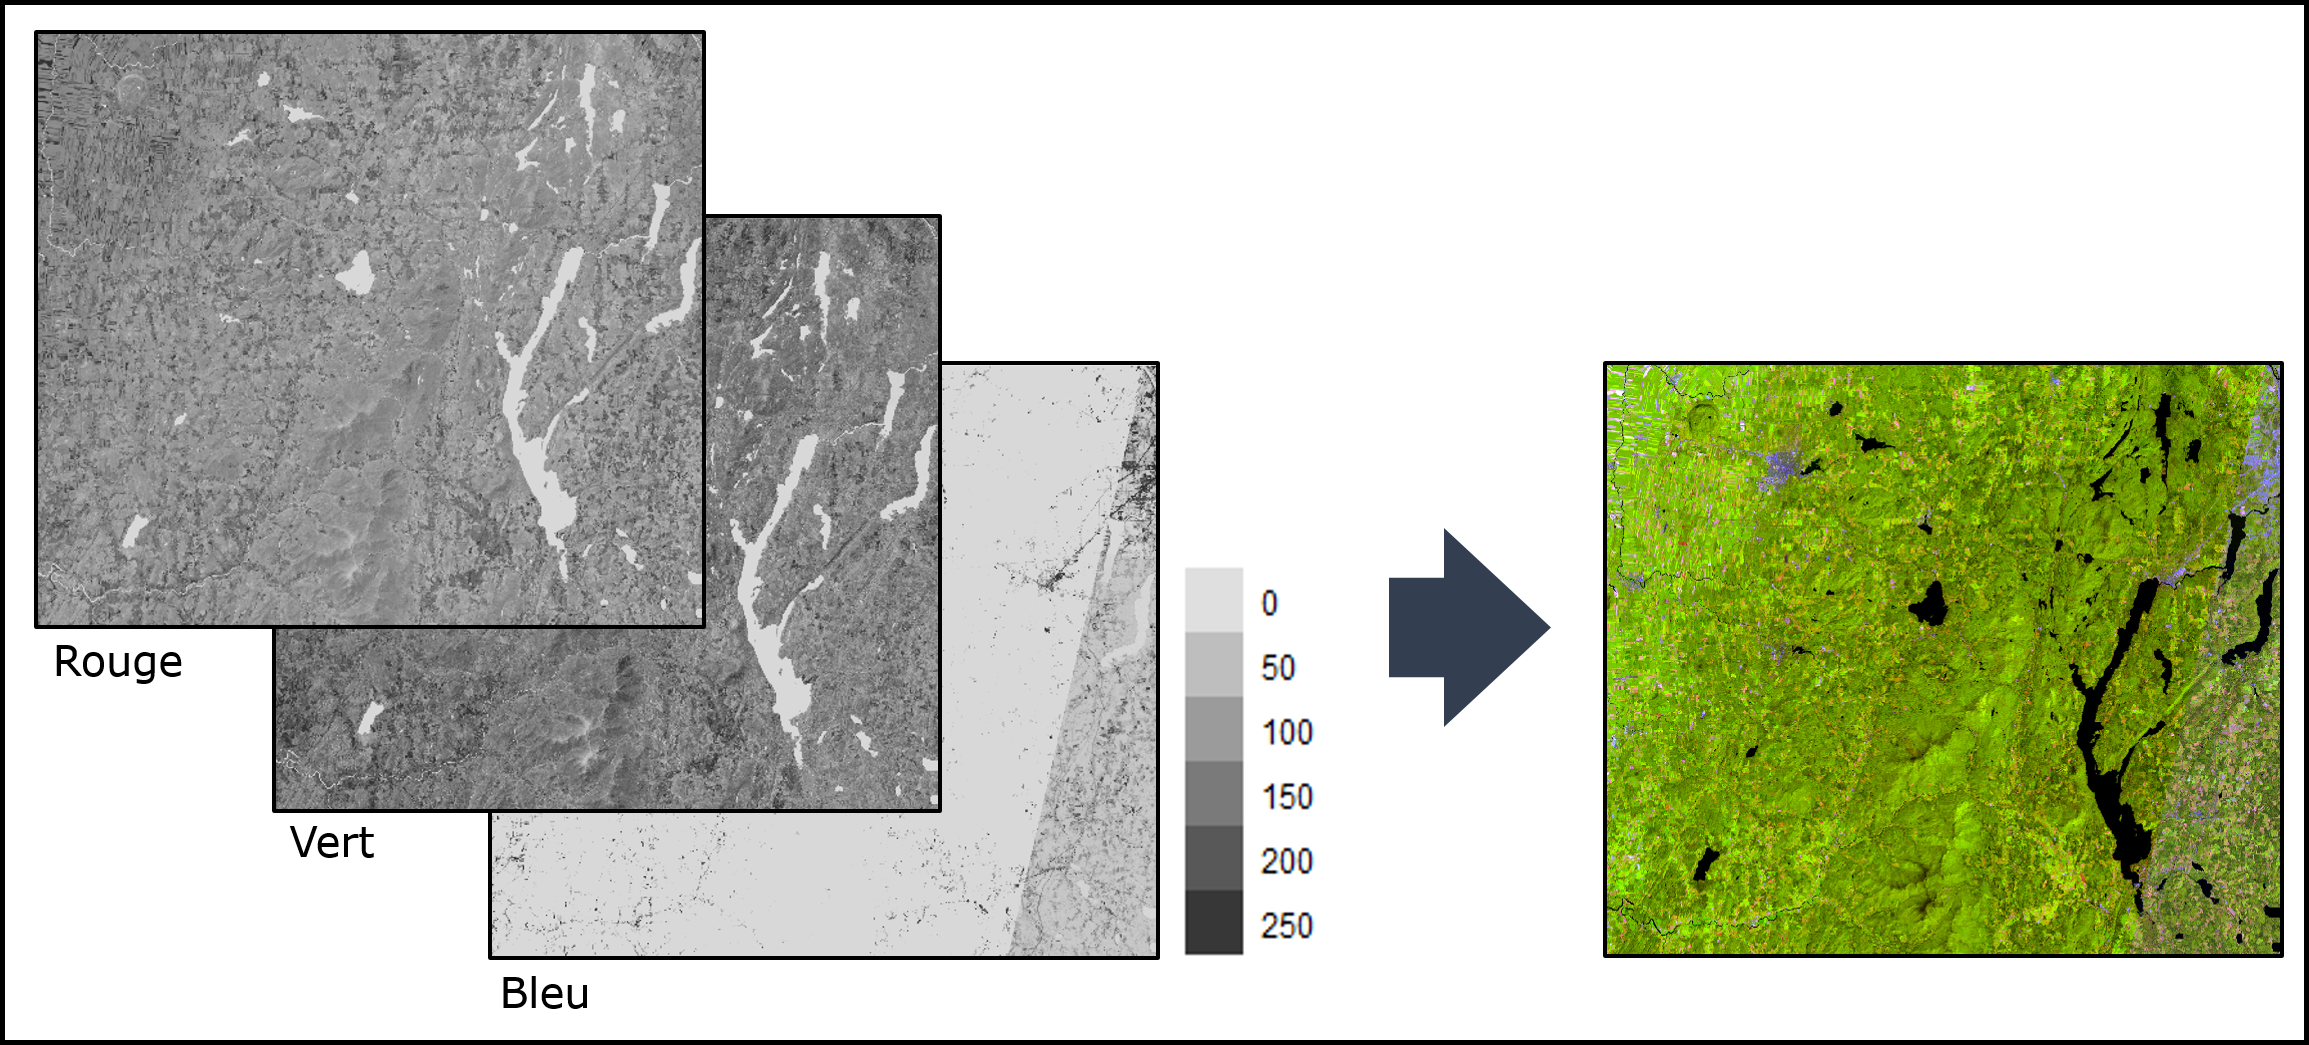
\includegraphics[width=1\linewidth]{Module2/images/2_3bands} \hfill{}

\caption{Image satellitaire de région de l’Estrie. Le raster multi-bande contient une bande de rouge, une bande de vert et une bande de bleu. L’image couleur s’obtient en combinant les trois bandes.  Source de données: https://mern.gouv.qc.ca/nos-publications/spatiocarte-quebec/}\label{fig:3bands}
\end{figure}

\hypertarget{format-des-donnuxe9es-matricielles}{%
\paragraph{Format des données matricielles}\label{format-des-donnuxe9es-matricielles}}
\addcontentsline{toc}{paragraph}{Format des données matricielles}

Tout comme les données vectorielles, les données matricielles peuvent être stockées dans une grande variété de formats différents. Les images possèdent des structures matricielles, ainsi les formats bien connus pour la transmission d'images sur le Web, .jpg (Joint Photographic Experts Group), .gif (Graphics Interchange Format), et .png (Portable Network Graphics), sont des exemples de format de données matricielles.

Voici une liste non-exhaustive de formats de données matricielles.

\begin{quote}
GRID (.GRD)
\end{quote}

GRID est le format propriétaire d'ESRI pour stocker des données matricielles.

\begin{quote}
TIFF AND GEOTIFF (.TIF)
\end{quote}

Le Tag Image File format (TIFF) est utilisé pour le stockage d'images numériques. Il a la particularité d'être comme un contenant dans lequel plusieurs informations additionnelles sur les données peuvent être stockées (par ex. les attributs, et autres métadonnées).
Le format GeoTIFF est un fichier .tif standard dans lequel on intègre des informations additionnelles sur la localisation spatiale des données (p.~ex. la résolution, l'étendue ou le système de coordonnées géographiques).

\begin{quote}
COMMA SEPERATED VALUE FORTMAT (.CSV)
\end{quote}

Le format .csv contient du texte séparé par des virgules, et correspond à une façon simple et très répandue de représenter des données matricielles. Par exemple, un fichier .csv pourrait être constitué de trois colonnes : la première pour la coordonnée x de la cellule, la deuxième pour sa coordonnée y, et la troisième pour la valeur de l'attribut.

Une autre façon d'utiliser le format .csv est d'y stocker la matrice de données sous forme d'un tableau de dimension égale à cette dernière. Chaque entrée du tableau donne la valeur d'attribut pour la cellule correspondante. Les informations sur la localisation spatiale doivent alors être fournies en en-tête du fichier.

\begin{quote}
BITMAP (.BMP)
\end{quote}

BITMAP est le format d'images utilisé dans les applications de Microsoft Windows.

De plus, comme expliqué plus haut, la géodatabase et Web Map Service sont aussi utilisés pour les données matricielles.

Peu importe le type de données spatiales et le format utilisé pour les stocker, les données spatiales sont souvent accompagnées de \textbf{métadonnées}. Les métadonnées sont les données sur les données. C'est-à-dire qu'elles viennent donner des informations supplémentaires pour faciliter la compréhension et l'utilisation des données spatiales (p.~ex. l'origine des données, l'auteur.e, les détails sur la structure, le lexique, les abréviations, la légende, etc.). Idéalement, tout ensemble de données devrait être accompagné de métadonnées.

\hypertarget{les-systuxe8mes-de-coordonnuxe9es-de-ruxe9fuxe9rence}{%
\subsection{Les systèmes de coordonnées de référence}\label{les-systuxe8mes-de-coordonnuxe9es-de-ruxe9fuxe9rence}}

\begin{itemize}
\tightlist
\item
  Coordonnées angulaires, projections, notations.
\end{itemize}

\hypertarget{exercice-1}{%
\section{Exercice}\label{exercice-1}}

\hypertarget{vec}{%
\chapter{Les données vectorielles}\label{vec}}

L'objectif principal de ce module est d'apprendre à lire, interpréter et visualiser des données vectorielles\footnote{L'ensemble du matériel disponible dans ce module est adapté du cours \emph{Introduction to Geospatial Raster and Vector Data with R} \citep{Data_Carpentry_IntroGeospatial} de l'organisme \href{https://datacarpentry.org/}{Data Carpentry}. Data Carpentry développe et offre des formations variées et spécialisées sur le traitement et l'analyse de données. Ses formations s'adressent surtout aux chercheuses et chercheurs scientifiques, mais peuvent être consultées par quiconque car leur matériel est libre d'accès. N'hésitez donc pas à y jeter un coup d'œil.}

À la fin de ce module vous saurez:

\begin{itemize}
\tightlist
\item
  Lire un \emph{shapefile}, explorer ses métadonnées et interpréter sa géométrie.
\item
  Visualiser des données vectorielles de type point, ligne et polygone.
\item
  Visualiser des données vectorielles par attribut.
\item
  Visualiser plusieurs données vectorielles au sein d'une même figure.
\item
  Transformer le système de coordonnées de référence de données vectorielles.
\end{itemize}

Vous utiliserez les librairies suivantes:

\begin{itemize}
\tightlist
\item
  \texttt{sf}
\item
  \texttt{rgdal}
\item
  \texttt{dplyr}
\item
  \texttt{ggplot2}
\item
  \texttt{ggpubr}
\end{itemize}

Vous apprendrez à utiliser les fonctions suivantes:

\begin{itemize}
\tightlist
\item
  \texttt{st\_read()}, \texttt{st\_write()}
\item
  \texttt{st\_geometry\_type()}
\item
  \texttt{st\_crs()}
\item
  \texttt{st\_bbox()}
\item
  \texttt{geom\_sf}
\item
  \texttt{filter()}
\item
  \texttt{st\_transform()}
\item
  \texttt{ggarrange()}
\end{itemize}

Dans la section Leçon, vous utiliserez des données vectorielles relatives au réseau de pistes cyclables de la ville de Montréal et aux accidents routiers impliquant des bicyclettes.

Dans la section Exercice, vous utiliserez XXXXX

\hypertarget{leuxe7on-2}{%
\section{Leçon}\label{leuxe7on-2}}

Dans le cadre de cette leçon, nous allons explorer des données vectorielles relatives au réseau de pistes cyclables de la ville de Montréal et aux accidents routiers impliquant des bicyclettes.
Téléchargez les \href{https://github.com/elisefilotas/Donnees_spatiales/blob/master/Montreal_Velo.zip}{données sur le réseau de pistes cyclables}. Sauvegardez le dossier compressé (\texttt{zip}) dans votre répertoire de travail \texttt{Donnees} pour ce module, et dézippez-le. Le dossier Montreal\_Velo comprend trois sous-dossiers:

\begin{itemize}
\tightlist
\item
  \texttt{accidents}
\item
  \texttt{pistes}
\item
  \texttt{terre}.
\end{itemize}

\hypertarget{introduction-aux-donnuxe9es-vectorielles-sous-r}{%
\subsection{Introduction aux données vectorielles sous R}\label{introduction-aux-donnuxe9es-vectorielles-sous-r}}

\hypertarget{lire-un-shapefile-et-interpruxe9ter-sa-guxe9omuxe9trie}{%
\subsubsection*{\texorpdfstring{Lire un \emph{shapefile} et interpréter sa géométrie}{Lire un shapefile et interpréter sa géométrie}}\label{lire-un-shapefile-et-interpruxe9ter-sa-guxe9omuxe9trie}}


Pour lire des données vectorielles contenues dans un fichier \emph{shapefile}, nous allons utiliser la librairie \texttt{sf}. Notez que la librairie \texttt{rgdal} se charge automatiquement lorsque \texttt{sf} se charge.

\begin{Shaded}
\begin{Highlighting}[]
\KeywordTok{library}\NormalTok{(sf)}
\end{Highlighting}
\end{Shaded}

Nous allons lire les trois \emph{shapefiles} suivants :

\begin{itemize}
\tightlist
\item
  Des données vectorielles de type polygone représentant la frontière de notre zone d'étude, ici, l'île de Montréal.
\item
  Des données vectorielles de type ligne représentant les pistes cyclables sur l'île de Montréal, et
\item
  Des données vectorielles de type point représentant la position d'accidents impliquant des bicyclettes.
\end{itemize}

Dans un premier temps, nous allons ouvrir les données vectorielles de type polygone qui contiennent les limites terrestres de l'île de Montréal. Pour lire ces données nous utiliserons la fonction \texttt{st\_read()} de la librarie \texttt{sf}. Pour utiliser \texttt{st\_read()} nous devons spécifier le chemin menant au fichier \emph{shapefile} à lire.

\begin{Shaded}
\begin{Highlighting}[]
\NormalTok{chemin<-}\StringTok{"D:/votrechemin/SCI1031/Module3/Donnees/"}
\NormalTok{nom_du_fichier <-}\StringTok{ }\KeywordTok{paste}\NormalTok{(chemin, }\StringTok{"/Montreal_Velo/terre/terre_shp.shp"}\NormalTok{, }\DataTypeTok{sep =} \StringTok{""}\NormalTok{)}
\NormalTok{limites_terrestres <-}\StringTok{ }\KeywordTok{st_read}\NormalTok{(nom_du_fichier)}
\end{Highlighting}
\end{Shaded}

\begin{verbatim}
Reading layer `terre_shp' from data source `/home/kevcaz/Github/Books/sci1031/Module3/data/Montreal_Velo/terre/terre_shp.shp' using driver `ESRI Shapefile'
Simple feature collection with 72 features and 1 field
geometry type:  POLYGON
dimension:      XY
bbox:           xmin: 267500 ymin: 5029000 xmax: 306700 ymax: 5063000
CRS:            32188
\end{verbatim}

La fonction \texttt{st\_read()} vous permet d'ores et déjà d'obtenir certaines informations sur la structure des données vectorielles que vous venez de lire: le type de géométrie (\texttt{geometry\ type}), la dimension des données (\texttt{dimension}), l'étendue spatiale des données (\texttt{bbox}), et les informations relatives au système de coordonnées de référence, le SPSG (\texttt{epsg\ (SRID)}) et la projection (\texttt{proj4string}). Nous explorerons ces propriétés en détails plus bas.

Nous allons maintenant lire les données vectorielles de type ligne, en utilisant encore la fonction \texttt{st\_read()}.

\begin{Shaded}
\begin{Highlighting}[]
\NormalTok{chemin <-}\StringTok{"D:/votrechemin/SCI1031/Module3/Donnees/"}
\NormalTok{nom_du_fichier<-}\StringTok{ }\KeywordTok{paste}\NormalTok{(chemin, }\StringTok{"/Montreal_Velo/pistes/pistes_cyclables_type.shp"}\NormalTok{, }\DataTypeTok{sep =} \StringTok{""}\NormalTok{)}
\NormalTok{pistes_cyclables <-}\StringTok{ }\KeywordTok{st_read}\NormalTok{(nom_du_fichier)}
\end{Highlighting}
\end{Shaded}

\begin{verbatim}
Reading layer `pistes_cyclables_type' from data source `/home/kevcaz/Github/Books/sci1031/Module3/data/Montreal_Velo/pistes/pistes_cyclables_type.shp' using driver `ESRI Shapefile'
Simple feature collection with 6395 features and 1 field
geometry type:  MULTILINESTRING
dimension:      XY
bbox:           xmin: 268000 ymin: 5029000 xmax: 306300 ymax: 5063000
CRS:            32188
\end{verbatim}

Finalement, nous allons lire les données vectorielles de type point, en utilisant toujours la fonction \texttt{st\_read()}.

\begin{Shaded}
\begin{Highlighting}[]
\NormalTok{chemin<-}\StringTok{"D:/votrechemin/SCI1031/Module3/Donnees/"}
\NormalTok{nom_du_fichier<-}\StringTok{ }\KeywordTok{paste}\NormalTok{(chemin, }\StringTok{"/Montreal_Velo/accidents/accidents2018_Mtl_velo.shp"}\NormalTok{, }\DataTypeTok{sep =} \StringTok{""}\NormalTok{)}
\NormalTok{pistes_cyclables <-}\StringTok{ }\KeywordTok{st_read}\NormalTok{(nom_du_fichier)}
\end{Highlighting}
\end{Shaded}

\begin{Shaded}
\begin{Highlighting}[]
\NormalTok{accidents_velo <-}\StringTok{ }\KeywordTok{st_read}\NormalTok{(}\StringTok{"Module3/data/Montreal_Velo/accidents/accidents2018_Mtl_velo.shp"}\NormalTok{)}
\end{Highlighting}
\end{Shaded}

\begin{verbatim}
Reading layer `accidents2018_Mtl_velo' from data source `/home/kevcaz/Github/Books/sci1031/Module3/data/Montreal_Velo/accidents/accidents2018_Mtl_velo.shp' using driver `ESRI Shapefile'
Simple feature collection with 796 features and 1 field
geometry type:  POINT
dimension:      XY
bbox:           xmin: 269500 ymin: 5030000 xmax: 305400 ymax: 5059000
CRS:            32188
\end{verbatim}

Remarquez que le type de géométrie (\texttt{geometry\ type}) diffère pour les trois classes de données lues comme nous nous y attendions.

\#\#\#\#Explorer les métadonnées d'un \emph{shapefile} \{-\}

Les informations contenues dans un \emph{shapefile} sont appelées des métadonnées. Nous sommes particulièrement intéressées aux métadonnées géospatiales.

Les métadonnées fondamentales d'un \emph{shapefile} sont :

\begin{enumerate}
\def\labelenumi{\arabic{enumi}.}
\tightlist
\item
  Le type de géométrie : le type de classes des données vectorielles téléchargées.
\item
  La projection : le système de coordonnées de référence utilisé pour représenter les données.
\item
  L'étendue spatiale : la superficie géographique couvrant les données vectorielles.
\end{enumerate}

Nous pouvons explorer chacune de ces métadonnées en utilisant des fonctions de la librairie \texttt{sf}. Le type de géométrie est obtenu par la fonction \texttt{st\_geometry\_type()}. Par exemple, pour les limites terrestres de la ville de Montréal, cette fonction nous donne:

\begin{Shaded}
\begin{Highlighting}[]
\KeywordTok{st_geometry_type}\NormalTok{(limites_terrestres)}
\end{Highlighting}
\end{Shaded}

\begin{verbatim}
 [1] POLYGON POLYGON POLYGON POLYGON POLYGON POLYGON
 [7] POLYGON POLYGON POLYGON POLYGON POLYGON POLYGON
[13] POLYGON POLYGON POLYGON POLYGON POLYGON POLYGON
[19] POLYGON POLYGON POLYGON POLYGON POLYGON POLYGON
[25] POLYGON POLYGON POLYGON POLYGON POLYGON POLYGON
[31] POLYGON POLYGON POLYGON POLYGON POLYGON POLYGON
[37] POLYGON POLYGON POLYGON POLYGON POLYGON POLYGON
[43] POLYGON POLYGON POLYGON POLYGON POLYGON POLYGON
[49] POLYGON POLYGON POLYGON POLYGON POLYGON POLYGON
[55] POLYGON POLYGON POLYGON POLYGON POLYGON POLYGON
[61] POLYGON POLYGON POLYGON POLYGON POLYGON POLYGON
[67] POLYGON POLYGON POLYGON POLYGON POLYGON POLYGON
18 Levels: GEOMETRY POINT LINESTRING ... TRIANGLE
\end{verbatim}

Nous avons ainsi la confirmation que ces données vectorielles correspondent à des polygones (plus exactement, 72 polygones). Les 18 niveaux donnés en dessous constituent une liste des classes possibles de géométrie.

En comparaison, pour les données de type ligne et de type point nous obtenons plutôt :

\begin{Shaded}
\begin{Highlighting}[]
\KeywordTok{st_geometry_type}\NormalTok{(pistes_cyclables)}
\end{Highlighting}
\end{Shaded}

\begin{verbatim}
   [1] MULTILINESTRING MULTILINESTRING MULTILINESTRING
   [4] MULTILINESTRING MULTILINESTRING MULTILINESTRING
...
 [ reached getOption("max.print") -- omitted 3995 entries ]
18 Levels: GEOMETRY POINT LINESTRING ... TRIANGLE
\end{verbatim}

\begin{Shaded}
\begin{Highlighting}[]
\KeywordTok{st_geometry_type}\NormalTok{(accidents_velo)}
\end{Highlighting}
\end{Shaded}

\begin{verbatim}
  [1] POINT POINT POINT POINT POINT POINT POINT POINT
  [9] POINT POINT POINT POINT POINT POINT POINT POINT
...
[793] POINT POINT POINT POINT
18 Levels: GEOMETRY POINT LINESTRING ... TRIANGLE
\end{verbatim}

Vous remarquez alors que les pistes cyclables sont composées de nombreuses multilignes. Une multiligne étant elle-même un ensemble de lignes.
Quant aux accidents de vélo, ce sont des points qui désignent la position précise des accidents. On en compte 796 en 2018.

Vérifions maintenant la projection des \emph{shapefiles} en utilisant la fonction \texttt{st\_crs()} de la librarie \texttt{sf}:

\begin{Shaded}
\begin{Highlighting}[]
\KeywordTok{st_crs}\NormalTok{(limites_terrestres)}
\end{Highlighting}
\end{Shaded}

\begin{verbatim}
Coordinate Reference System:
  User input: 32188 
  wkt:
PROJCS["NAD83 / MTM zone 8",
    GEOGCS["NAD83",
        DATUM["North_American_Datum_1983",
            SPHEROID["GRS 1980",6378137,298.257222101,
                AUTHORITY["EPSG","7019"]],
            TOWGS84[0,0,0,0,0,0,0],
            AUTHORITY["EPSG","6269"]],
        PRIMEM["Greenwich",0,
            AUTHORITY["EPSG","8901"]],
        UNIT["degree",0.0174532925199433,
            AUTHORITY["EPSG","9122"]],
        AUTHORITY["EPSG","4269"]],
    PROJECTION["Transverse_Mercator"],
    PARAMETER["latitude_of_origin",0],
    PARAMETER["central_meridian",-73.5],
    PARAMETER["scale_factor",0.9999],
    PARAMETER["false_easting",304800],
    PARAMETER["false_northing",0],
    UNIT["metre",1,
        AUTHORITY["EPSG","9001"]],
    AXIS["E(X)",EAST],
    AXIS["N(Y)",NORTH],
    AUTHORITY["EPSG","32188"]]
\end{verbatim}

\begin{Shaded}
\begin{Highlighting}[]
\KeywordTok{st_crs}\NormalTok{(pistes_cyclables)}
\end{Highlighting}
\end{Shaded}

\begin{verbatim}
Coordinate Reference System:
  User input: 32188 
  wkt:
PROJCS["NAD83 / MTM zone 8",
    GEOGCS["NAD83",
        DATUM["North_American_Datum_1983",
            SPHEROID["GRS 1980",6378137,298.257222101,
                AUTHORITY["EPSG","7019"]],
            TOWGS84[0,0,0,0,0,0,0],
            AUTHORITY["EPSG","6269"]],
        PRIMEM["Greenwich",0,
            AUTHORITY["EPSG","8901"]],
        UNIT["degree",0.0174532925199433,
            AUTHORITY["EPSG","9122"]],
        AUTHORITY["EPSG","4269"]],
    PROJECTION["Transverse_Mercator"],
    PARAMETER["latitude_of_origin",0],
    PARAMETER["central_meridian",-73.5],
    PARAMETER["scale_factor",0.9999],
    PARAMETER["false_easting",304800],
    PARAMETER["false_northing",0],
    UNIT["metre",1,
        AUTHORITY["EPSG","9001"]],
    AXIS["E(X)",EAST],
    AXIS["N(Y)",NORTH],
    AUTHORITY["EPSG","32188"]]
\end{verbatim}

\begin{Shaded}
\begin{Highlighting}[]
\KeywordTok{st_crs}\NormalTok{(accidents_velo)}
\end{Highlighting}
\end{Shaded}

\begin{verbatim}
Coordinate Reference System:
  User input: 32188 
  wkt:
PROJCS["NAD83 / MTM zone 8",
    GEOGCS["NAD83",
        DATUM["North_American_Datum_1983",
            SPHEROID["GRS 1980",6378137,298.257222101,
                AUTHORITY["EPSG","7019"]],
            TOWGS84[0,0,0,0,0,0,0],
            AUTHORITY["EPSG","6269"]],
        PRIMEM["Greenwich",0,
            AUTHORITY["EPSG","8901"]],
        UNIT["degree",0.0174532925199433,
            AUTHORITY["EPSG","9122"]],
        AUTHORITY["EPSG","4269"]],
    PROJECTION["Transverse_Mercator"],
    PARAMETER["latitude_of_origin",0],
    PARAMETER["central_meridian",-73.5],
    PARAMETER["scale_factor",0.9999],
    PARAMETER["false_easting",304800],
    PARAMETER["false_northing",0],
    UNIT["metre",1,
        AUTHORITY["EPSG","9001"]],
    AXIS["E(X)",EAST],
    AXIS["N(Y)",NORTH],
    AUTHORITY["EPSG","32188"]]
\end{verbatim}

Les données de tous les \emph{shapefiles} sont dans la projection de Mercator transverse (\texttt{+proj=tmerc}) et utilisent le Système de référence géodésique nord-américan de 1983 (\texttt{+datum=NAD83}). Il n'y a pas de EPSG assigné à ces données. Connaitre le SCR est essentiel pour interpréter l'étendue spatiale des objets spatiaux puisque celui-ci précise, en quelque sorte, les unités de mesure.

Pour connaître l'étendue spatiale des \emph{shapefiles}, nous utilisons la fonction \texttt{st\_bbox()} de la librairie \texttt{sf} :

\begin{Shaded}
\begin{Highlighting}[]
\KeywordTok{st_bbox}\NormalTok{(limites_terrestres)}
\end{Highlighting}
\end{Shaded}

\begin{verbatim}
   xmin    ymin    xmax    ymax 
 267517 5029232  306669 5062642 
\end{verbatim}

\begin{Shaded}
\begin{Highlighting}[]
\KeywordTok{st_bbox}\NormalTok{(pistes_cyclables)}
\end{Highlighting}
\end{Shaded}

\begin{verbatim}
   xmin    ymin    xmax    ymax 
 267984 5029291  306349 5062582 
\end{verbatim}

\begin{Shaded}
\begin{Highlighting}[]
\KeywordTok{st_bbox}\NormalTok{(accidents_velo)}
\end{Highlighting}
\end{Shaded}

\begin{verbatim}
   xmin    ymin    xmax    ymax 
 269489 5029752  305368 5059058 
\end{verbatim}

L'étendue spatiale d'un \emph{shapefile} ou d'un objet spatial dans \texttt{R} représente les limites géographiques des données, ou la localisation des données les plus au sud, nord, est et ouest.

ICI BESOIN D'UNE FIGURE COMME CELLE DE NEON

Finalement, nous pouvons visualiser toutes les métadonnées et les attributs d'un \emph{shapefile} simplement en écrivant son nom dans la console \texttt{R}:

\begin{Shaded}
\begin{Highlighting}[]
\NormalTok{limites_terrestres}
\end{Highlighting}
\end{Shaded}

\begin{verbatim}
Simple feature collection with 72 features and 1 field
geometry type:  POLYGON
dimension:      XY
bbox:           xmin: 267500 ymin: 5029000 xmax: 306700 ymax: 5063000
CRS:            32188
First 10 features:
   DefaultAtt                       geometry
1        <NA> POLYGON ((299608 5038364, 2...
2        <NA> POLYGON ((301350 5036978, 3...
3        <NA> POLYGON ((300403 5038997, 3...
4        <NA> POLYGON ((300744 5039496, 3...
5        <NA> POLYGON ((302032 5043372, 3...
6        <NA> POLYGON ((302299 5043145, 3...
7        <NA> POLYGON ((302508 5040978, 3...
8        <NA> POLYGON ((304719 5062024, 3...
9        <NA> POLYGON ((304927 5062499, 3...
10       <NA> POLYGON ((305396 5062622, 3...
\end{verbatim}

\begin{Shaded}
\begin{Highlighting}[]
\NormalTok{pistes_cyclables}
\end{Highlighting}
\end{Shaded}

\begin{verbatim}
Simple feature collection with 6395 features and 1 field
geometry type:  MULTILINESTRING
dimension:      XY
bbox:           xmin: 268000 ymin: 5029000 xmax: 306300 ymax: 5063000
CRS:            32188
First 10 features:
                       TYPE_VOIE
1         Piste cyclable sur rue
2  Piste cyclable en site propre
3              Chaussée désignée
4                 Bande cyclable
5  Piste cyclable en site propre
6  Piste cyclable en site propre
7  Piste cyclable en site propre
8              Chaussée désignée
9  Piste cyclable en site propre
10 Piste cyclable en site propre
                         geometry
1  MULTILINESTRING ((297752 50...
2  MULTILINESTRING ((305050 50...
3  MULTILINESTRING ((299076 50...
4  MULTILINESTRING ((287779 50...
5  MULTILINESTRING ((300752 50...
6  MULTILINESTRING ((300953 50...
7  MULTILINESTRING ((299010 50...
8  MULTILINESTRING ((276415 50...
9  MULTILINESTRING ((293077 50...
10 MULTILINESTRING ((304787 50...
\end{verbatim}

\begin{Shaded}
\begin{Highlighting}[]
\NormalTok{accidents_velo}
\end{Highlighting}
\end{Shaded}

\begin{verbatim}
Simple feature collection with 796 features and 1 field
geometry type:  POINT
dimension:      XY
bbox:           xmin: 269500 ymin: 5030000 xmax: 305400 ymax: 5059000
CRS:            32188
First 10 features:
   FID               geometry
1    0 POINT (279673 5041015)
2    1 POINT (277292 5039169)
3    2 POINT (275581 5036314)
4    3 POINT (274728 5035946)
5    4 POINT (283935 5040875)
6    5 POINT (280442 5039871)
7    6 POINT (279626 5040700)
8    7 POINT (277734 5038853)
9    8 POINT (276487 5038090)
10   9 POINT (278357 5040125)
\end{verbatim}

\hypertarget{visualisation-de-shapefiles-sous-r}{%
\subsection{\texorpdfstring{Visualisation de \emph{shapefiles} sous R}{Visualisation de shapefiles sous R}}\label{visualisation-de-shapefiles-sous-r}}

\hypertarget{visualiser-des-donnuxe9es-vectorielles}{%
\subsubsection*{Visualiser des données vectorielles}\label{visualiser-des-donnuxe9es-vectorielles}}


Vous allez maintenant apprendre à visualer des données \emph{shapefile} en utilisant la fonction \texttt{ggplot()} de la librairie \texttt{ggplot2}.

\begin{Shaded}
\begin{Highlighting}[]
\KeywordTok{library}\NormalTok{(ggplot2)}
\end{Highlighting}
\end{Shaded}

Dans un premier temps, visualisons les limites terrestres de l'île de Montréal (Fig \ref{fig:plot-terre}).

\begin{Shaded}
\begin{Highlighting}[]
\KeywordTok{ggplot}\NormalTok{() }\OperatorTok{+}
\KeywordTok{geom_sf}\NormalTok{(}\DataTypeTok{data =}\NormalTok{ limites_terrestres, }\DataTypeTok{size =} \DecValTok{1}\NormalTok{, }\DataTypeTok{color =} \StringTok{"black"}\NormalTok{, }\DataTypeTok{fill =} \StringTok{"white"}\NormalTok{) }\OperatorTok{+}
\KeywordTok{ggtitle}\NormalTok{(}\StringTok{"Limites terrestres de l'île de Montréal"}\NormalTok{)}
\end{Highlighting}
\end{Shaded}

\begin{figure}

{\centering 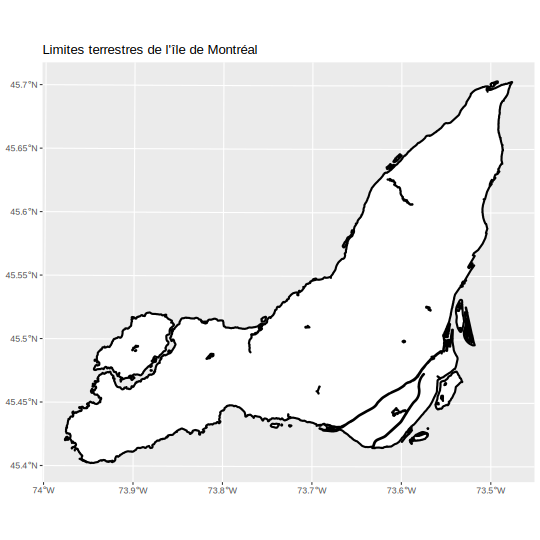
\includegraphics[width=540px]{Cours_SpatialR_files/figure-latex/plot-terre-1} 

}

\caption{Limites terrestres de l'île de Montréal}\label{fig:plot-terre}
\end{figure}

La fonction \texttt{geom\_sf()} permet de faire des représentations simples d'objets vectoriels de géométrie de type point, ligne et polygone.
Cette fonction peut prendre plusieurs arguments\footnote{Pour plus d'information sur la fonction \texttt{geom\_sf}, consultez le chapitre \href{https://ggplot2.tidyverse.org/reference/ggsf.html}{Visualise sf objects} \citep{Wickham_ggplot2_2016}}. Les arguments utilisés ici sont:

\begin{itemize}
\tightlist
\item
  les données (\texttt{data})
\item
  la taille du trait avec laquelle on illustre l'objet (\texttt{size})
\item
  la couleur du trait, et la couleur de la surface délimitée par le trait (\texttt{color}).
\end{itemize}

La fonction ggtitle permet d'ajouter un titre à la figure générée.

Remarquez que chaque fonction est écrite sur sa propre ligne, pour faciliter la lecture des lignes de commande, et que chaque fonction qui s'ajoute à \texttt{ggplot()} est précédée par le signe plus \texttt{+}.

Dans un deuxième temps, visualisons les pistes cyclables (Fig \ref{fig:plot-velo}).

\begin{Shaded}
\begin{Highlighting}[]
\KeywordTok{ggplot}\NormalTok{() }\OperatorTok{+}
\KeywordTok{geom_sf}\NormalTok{(}\DataTypeTok{data =}\NormalTok{ pistes_cyclables, }\DataTypeTok{size =} \DecValTok{1}\NormalTok{, }\DataTypeTok{color =} \StringTok{"darkgreen"}\NormalTok{) }\OperatorTok{+}
\KeywordTok{ggtitle}\NormalTok{(}\StringTok{"Pistes cyclables sur l'île de Montréal"}\NormalTok{)}
\end{Highlighting}
\end{Shaded}

\begin{figure}

{\centering 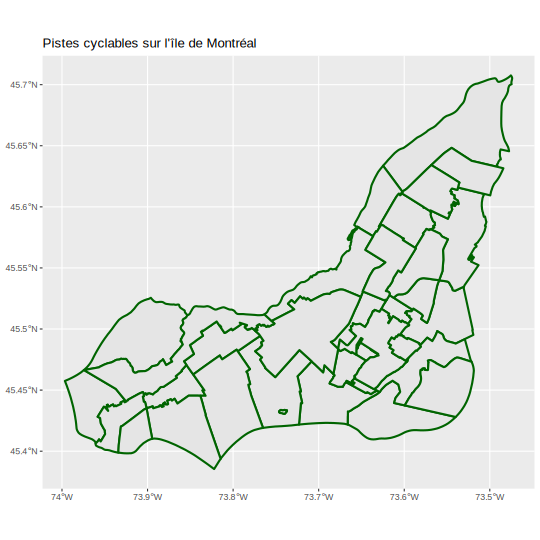
\includegraphics[width=540px]{Cours_SpatialR_files/figure-latex/plot-velo-1} 

}

\caption{Pistes cyclables sur l'île de Montréal}\label{fig:plot-velo}
\end{figure}

Pour visualiser des lignes, nous n'avons évidemment pas besoin de définir l'argument \texttt{fill} car nous visualisons des lignes plutôt qu'une surface. Vous remarquerez que les lignes, cette fois, sont vertes foncées (\texttt{darkgreen}).

Il existe 657 couleurs prédéfinies dans \texttt{R}. Taper la commande \texttt{colors()} dans votre console \texttt{R} pour voir afficher le nom des couleurs. Celles-sont sont listées par ordre alphabétique sauf pour la première couleur, qui est le blanc (\texttt{white}). Ainsi, vous pouvez utiliser une couleur en assignant son nom ou son numéro. Pour produire la figure précédente, \texttt{color\ =\ "darkgreen"} aurait pu être remplacé par
\texttt{color\ =\ colors(){[}81{]}}. Essayez pour voir.

Les couleurs peuvent aussi être définies selon leur composition en rouge, vert et bleu sur un intervalle allant de 0 à 255 - ce qu'on nomme le vecteur RGB (red, green, blue). Par exemple, la couleur jaune est représentée par le vecteur RGB (255, 255, 0). La couleur verte foncée, utilisée précédemment, est, quant à elle, représentée par le vecteur RGB (0, 100, 0). Les couleurs peuvent aussi être exprimées selon le système de notation \href{https://fr.wikipedia.org/wiki/Syst\%C3\%A8me_hexad\%C3\%A9cimal}{hexadécimal}. La fonction \texttt{rgb} permet de traduire un vecteur de couleur RGB en notation hexadécimal. Ainsi, pour produire la figure précédente, nous aurions pu définir le vecteur \texttt{vert\_fonce\ =\ rgb(0,\ 100,\ 0,\ maxColorValue=255)}, et remplacer \texttt{color\ =\ "darkgreen"} par \texttt{color\ =\ vert\_fonce}. Essayez pour voir.

Pour en apprendre davantage sur les couleurs dans \texttt{R}, vous êtes invité à consulter le site \href{https://github.com/EarlGlynn/colorchart/wiki/Color-Chart-in-R}{Earl Glynn} et à conserver dans vos notes son \href{Module3/3_TableauCouleurs.pdf}{tableau synthèse des couleurs} dans \texttt{R}.

Finalement, visualisons les accidents de la route impliquant des bicyclettes (Fig \ref{fig:plot-accidents}).

\begin{Shaded}
\begin{Highlighting}[]
\KeywordTok{ggplot}\NormalTok{() }\OperatorTok{+}
\KeywordTok{geom_sf}\NormalTok{(}\DataTypeTok{data =}\NormalTok{ accidents_velo, }\DataTypeTok{pch =} \DecValTok{19}\NormalTok{, }\DataTypeTok{cex =} \FloatTok{1.25}\NormalTok{, }\DataTypeTok{color =} \StringTok{"red"}\NormalTok{) }\OperatorTok{+}
\KeywordTok{ggtitle}\NormalTok{(}\StringTok{"Accidents de la route avec cyclistes sur l'île de Montréal"}\NormalTok{)}
\end{Highlighting}
\end{Shaded}

\begin{figure}

{\centering 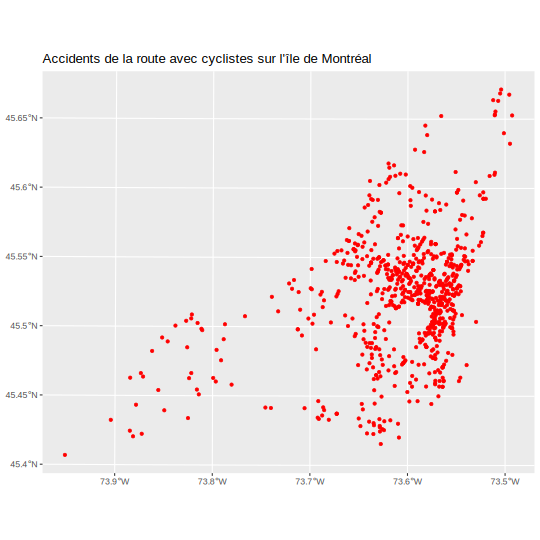
\includegraphics[width=540px]{Cours_SpatialR_files/figure-latex/plot-accidents-1} 

}

\caption{Accidents de la route avec cyclistes sur l'île de Montréal}\label{fig:plot-accidents}
\end{figure}

Le symbole utilisé pour illustrer la position des accidents est défini par l'argument \texttt{pch\ =\ 19}. Il existe 25 formats de points différents prédéfinis dans \texttt{R}. Les voici:

\begin{figure}

{\centering 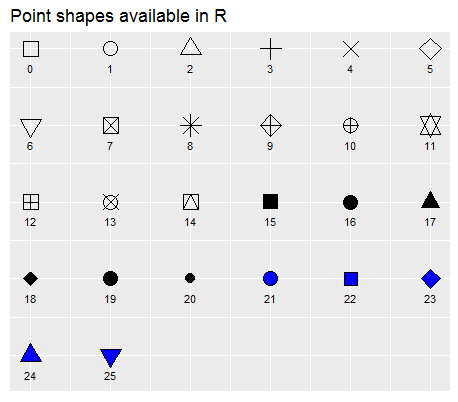
\includegraphics[width=0.5\linewidth]{Module3/3_symbolesR} 

}

\caption{Symboles disponibles}\label{fig:plot-symbols}
\end{figure}

L'argument \texttt{cex}, quant à lui, indique le facteur par lequel la taille du symbole sera augmentée ou réduite par rapport à 1, la valeur par défaut. Par exemple, `cex = 1.5' indique que le symbole sera 50\% plus grand, alors que 0.5 indique que le symbole sera 50\% plus petit.

Ainsi, nous pouvons changer les valeurs de ces arguments et représenter les accidents de vélo par des triangles oranges (Fig \ref{fig:plot-accidents2}).

\begin{Shaded}
\begin{Highlighting}[]
\KeywordTok{ggplot}\NormalTok{() }\OperatorTok{+}
\KeywordTok{geom_sf}\NormalTok{(}\DataTypeTok{data =}\NormalTok{ accidents_velo, }\DataTypeTok{pch =} \DecValTok{24}\NormalTok{, }\DataTypeTok{cex =} \FloatTok{1.5}\NormalTok{, }\DataTypeTok{color =} \StringTok{"black"}\NormalTok{, }\DataTypeTok{fill =} \StringTok{"orange"}\NormalTok{) }\OperatorTok{+}
\KeywordTok{ggtitle}\NormalTok{(}\StringTok{"Accidents de la route avec cyclistes sur l'île de Montréal"}\NormalTok{)}
\end{Highlighting}
\end{Shaded}

\begin{figure}

{\centering 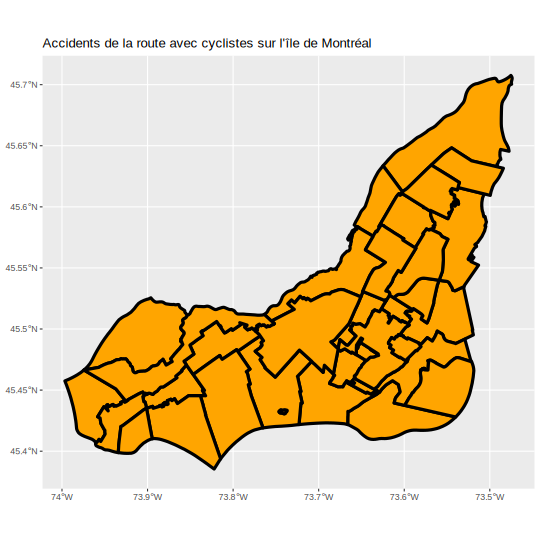
\includegraphics[width=540px]{Cours_SpatialR_files/figure-latex/plot-accidents2-1} 

}

\caption{Symbole et couleur différents pour illustrer les accidents de la route avec cyclistes sur l'île de Montréal}\label{fig:plot-accidents2}
\end{figure}

\hypertarget{visualiser-des-donnuxe9es-vectorielles-par-attribut}{%
\subsubsection*{Visualiser des données vectorielles par attribut}\label{visualiser-des-donnuxe9es-vectorielles-par-attribut}}


Lorsque nous avons affiché les métadonnées du \emph{shapefile} \texttt{pistes\_cyclables}, vous avez peut-être observé que ce dernier comprenait l'attribut \texttt{TYPE\_VOIE} qui caractérise le type de pistes cyclables de chaque multiligne. Affichons les métadonnées à nouveau:

\begin{Shaded}
\begin{Highlighting}[]
\NormalTok{pistes_cyclables}
\end{Highlighting}
\end{Shaded}

\begin{verbatim}
Simple feature collection with 6395 features and 1 field
geometry type:  MULTILINESTRING
dimension:      XY
bbox:           xmin: 268000 ymin: 5029000 xmax: 306300 ymax: 5063000
CRS:            32188
First 10 features:
                       TYPE_VOIE
1         Piste cyclable sur rue
2  Piste cyclable en site propre
3              Chaussée désignée
4                 Bande cyclable
5  Piste cyclable en site propre
6  Piste cyclable en site propre
7  Piste cyclable en site propre
8              Chaussée désignée
9  Piste cyclable en site propre
10 Piste cyclable en site propre
                         geometry
1  MULTILINESTRING ((297752 50...
2  MULTILINESTRING ((305050 50...
3  MULTILINESTRING ((299076 50...
4  MULTILINESTRING ((287779 50...
5  MULTILINESTRING ((300752 50...
6  MULTILINESTRING ((300953 50...
7  MULTILINESTRING ((299010 50...
8  MULTILINESTRING ((276415 50...
9  MULTILINESTRING ((293077 50...
10 MULTILINESTRING ((304787 50...
\end{verbatim}

Utilisons la fonction \texttt{levels} pour connaître ces types de voie cyclables. La fonction \texttt{levels} donne les différentes valeurs que peuvent prendre un attribut.

\begin{Shaded}
\begin{Highlighting}[]
\KeywordTok{levels}\NormalTok{(pistes_cyclables}\OperatorTok{$}\NormalTok{TYPE_VOIE)}
\end{Highlighting}
\end{Shaded}

\begin{verbatim}
[1] "Bande cyclable"                      
[2] "Chaussée désignée"                   
[3] "Piste cyclable au niveau du trottoir"
[4] "Piste cyclable en site propre"       
[5] "Piste cyclable sur rue"              
[6] "Sentier polyvalent"                  
\end{verbatim}

Si vous ne connaissez pas la distinction entre ces types d'aménagement cyclable, consulter ce \href{Module3/3_Amenagement3Cyclable3Mtl.pdf}{document sommaire} de la \emph{Ville de Montréal}\footnote{Ville de Montréal. Aménagements cyclables. Repéré le 19 mars 2020}

Nous voulons maintenant représenter les données vectorielles associées aux pistes cyclables de type \texttt{"Bande\ cyclable"}. Pour représenter une valeur précise d'un attribut, nous utiliserons la fonction \texttt{filter} de la librarie \texttt{dplyr}. Commençons par charger cette librairie.

\begin{Shaded}
\begin{Highlighting}[]
\KeywordTok{library}\NormalTok{(dplyr)}
\end{Highlighting}
\end{Shaded}

Utilisons la fonction \texttt{filter} qui permet de filtrer l'ensemble des valeurs de l'attribut \texttt{TYPE\_VOIE}, pour ne retenir que les données dont la valeur est identique (ce qui s'exprime par l'opération \texttt{==}) à `\,``Bande cyclable''\,'. Nous nommerons ce sous-ensemble de données \texttt{Bande}.

\begin{Shaded}
\begin{Highlighting}[]
\NormalTok{Bande <-pistes_cyclables }\OperatorTok
\StringTok{  }\KeywordTok{filter}\NormalTok{(TYPE_VOIE }\OperatorTok{==}\StringTok{"Bande cyclable"}\NormalTok{)}
\end{Highlighting}
\end{Shaded}

Nous représentons ce sous-ensemble de données de la même manière que pour l'ensemble complet (Fig \ref{fig:plot-velo}).

\begin{Shaded}
\begin{Highlighting}[]
\KeywordTok{ggplot}\NormalTok{()}\OperatorTok{+}
\StringTok{  }\KeywordTok{geom_sf}\NormalTok{(}\DataTypeTok{data =}\NormalTok{ Bande,  }\DataTypeTok{size =} \DecValTok{1}\NormalTok{, }\DataTypeTok{color =} \StringTok{"darkgreen"}\NormalTok{)}\OperatorTok{+}
\StringTok{  }\KeywordTok{ggtitle}\NormalTok{(}\StringTok{"Pistes cyclables sur l'île de Montréal"}\NormalTok{, }\DataTypeTok{subtitle =} \StringTok{"Bande cyclable"}\NormalTok{)}
\end{Highlighting}
\end{Shaded}

\begin{figure}

{\centering 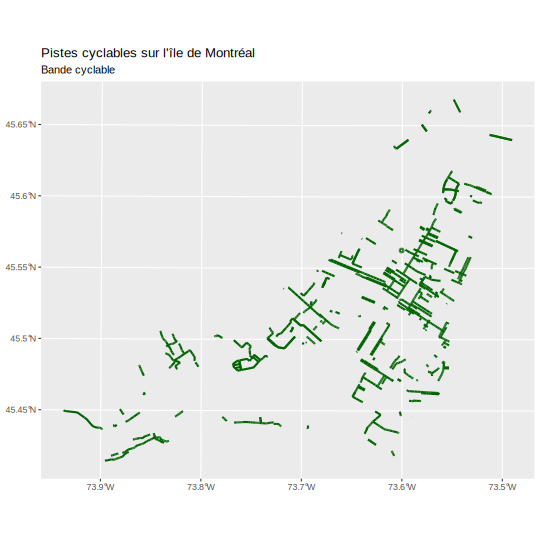
\includegraphics[width=540px]{Cours_SpatialR_files/figure-latex/plot-voie3-1} 

}

\caption{Bandes cyclables sur l'île de Montréal}\label{fig:plot-voie3}
\end{figure}

Nous voulons maintenant représenter les six types de voie cyclable par six couleurs différentes. Créons d'abord un vecteur de six couleurs, ce qu'on appelle une palette de couleurs.

\begin{Shaded}
\begin{Highlighting}[]
\NormalTok{couleurs_voie<-}\KeywordTok{c}\NormalTok{(}\StringTok{"darkgreen"}\NormalTok{, }\StringTok{"turquoise"}\NormalTok{, }\StringTok{"yellow"}\NormalTok{,}\StringTok{"darkblue"}\NormalTok{,}\StringTok{"violet"}\NormalTok{,}\StringTok{"orange"}\NormalTok{)}
\end{Highlighting}
\end{Shaded}

Nous pouvons demander à \texttt{ggplot} d'utiliser ces couleurs pour illustrer les différents types de voie cyclable (Fig \ref{fig:plot-voie5}).

\begin{Shaded}
\begin{Highlighting}[]
\KeywordTok{ggplot}\NormalTok{()}\OperatorTok{+}
\StringTok{  }\KeywordTok{geom_sf}\NormalTok{(}\DataTypeTok{data =}\NormalTok{ pistes_cyclables,  }\KeywordTok{aes}\NormalTok{(}\DataTypeTok{color =}\NormalTok{ TYPE_VOIE))}\OperatorTok{+}
\StringTok{  }\KeywordTok{scale_color_manual}\NormalTok{(}\DataTypeTok{values =}\NormalTok{ couleurs_voie)}\OperatorTok{+}
\StringTok{  }\KeywordTok{labs}\NormalTok{(}\DataTypeTok{color =} \StringTok{'Types de voie'}\NormalTok{)}\OperatorTok{+}
\StringTok{  }\KeywordTok{ggtitle}\NormalTok{(}\StringTok{"Pistes cyclables sur l'île de Montréal"}\NormalTok{, }\DataTypeTok{subtitle =} \StringTok{"Types de voie"}\NormalTok{)}
\end{Highlighting}
\end{Shaded}

\begin{figure}

{\centering 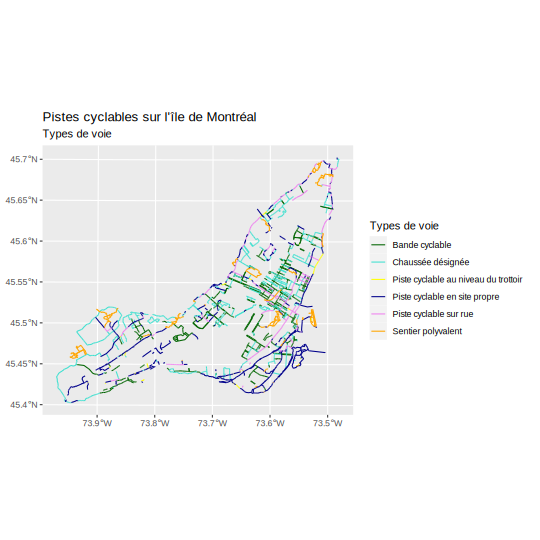
\includegraphics[width=540px]{Cours_SpatialR_files/figure-latex/plot-voie5-1} 

}

\caption{Types de voie cyclable sur l'île de Montréal}\label{fig:plot-voie5}
\end{figure}

La fonction \texttt{aes} décrit quelles variables dans les données (\texttt{data}) sont illustrées (dans notre exemple, ce sont \texttt{TYPE\_VOIE}) et par quelles
caractéristiques visuelles\footnote{Pour plus d'information sur la fonction \texttt{aes}, consultez le chapitre \href{https://ggplot2.tidyverse.org/reference/aes.html}{Construct aesthetic mappings} \citep{Wickham_ggplot2_2016}}. On nomme ces caractéristiques visuelles les ``esthétiques'' (\texttt{aes} pour ``aesthetic'' en anglais). Dans le présent exemple, nous nous préoccupons seulement de la couleur des données vectorielles, mais nous aurions pu aussi changer leur taille, le type de lignes, ou la forme des symboles (si la géométrie des données étaient de type point).

La fonction \texttt{scale\_color\_manual} permet de spécifier nos propres couleurs, sans quoi ce seront les couleurs par défaut qui seront utilisées\footnote{Pour plus d'information sur la fonction \texttt{scale\_colour\_manual}, consultez le chapitre \href{https://ggplot2.tidyverse.org/reference/scale_manual.html}{Create your own discrete scale} \citep{Wickham_ggplot2_2016}}.

Finalement, la fonction \texttt{labs} permet d'assigner un titre à la légende, sans quoi c'est le nom de la variable, telle que nous l'avons définie dans \texttt{R} qui sera affichée, ici, \texttt{TYPE\_VOIE}.

Nous pouvons aussi demander à \texttt{ggplot} de représenter les types de voie cyclable en utilisant différentes tailles de trait. De la même façon que précédemment, nous créons un vecteur de six tailles.

\begin{Shaded}
\begin{Highlighting}[]
\NormalTok{tailles_voie<-}\KeywordTok{c}\NormalTok{(}\DecValTok{1}\NormalTok{,}\FloatTok{1.2}\NormalTok{,}\FloatTok{1.5}\NormalTok{,}\FloatTok{1.7}\NormalTok{,}\DecValTok{2}\NormalTok{,}\FloatTok{2.2}\NormalTok{)}
\end{Highlighting}
\end{Shaded}

Puis représentatons les types de voie cyclable (Fig \ref{fig:plot-voie7}).

\begin{Shaded}
\begin{Highlighting}[]
\KeywordTok{ggplot}\NormalTok{()}\OperatorTok{+}
\StringTok{  }\KeywordTok{geom_sf}\NormalTok{(}\DataTypeTok{data =}\NormalTok{ pistes_cyclables,  }\KeywordTok{aes}\NormalTok{(}\DataTypeTok{color =}\NormalTok{ TYPE_VOIE, }\DataTypeTok{size =}\NormalTok{ TYPE_VOIE))}\OperatorTok{+}
\StringTok{  }\KeywordTok{scale_color_manual}\NormalTok{(}\DataTypeTok{values =}\NormalTok{ couleurs_voie)}\OperatorTok{+}
\StringTok{  }\KeywordTok{labs}\NormalTok{(}\DataTypeTok{color =} \StringTok{'Types de voie'}\NormalTok{)}\OperatorTok{+}
\StringTok{  }\KeywordTok{scale_size_manual}\NormalTok{(}\DataTypeTok{values =}\NormalTok{ tailles_voie)}\OperatorTok{+}
\StringTok{  }\KeywordTok{labs}\NormalTok{(}\DataTypeTok{size =} \StringTok{'Types de voie'}\NormalTok{)}\OperatorTok{+}
\StringTok{  }\KeywordTok{ggtitle}\NormalTok{(}\StringTok{"Pistes cyclables sur l'île de Montréal"}\NormalTok{, }\DataTypeTok{subtitle =} \StringTok{"Types de voie"}\NormalTok{)}\OperatorTok{+}
\StringTok{  }\KeywordTok{theme}\NormalTok{(}\DataTypeTok{legend.position =} \StringTok{"bottom"}\NormalTok{)}
\end{Highlighting}
\end{Shaded}

\begin{figure}

{\centering 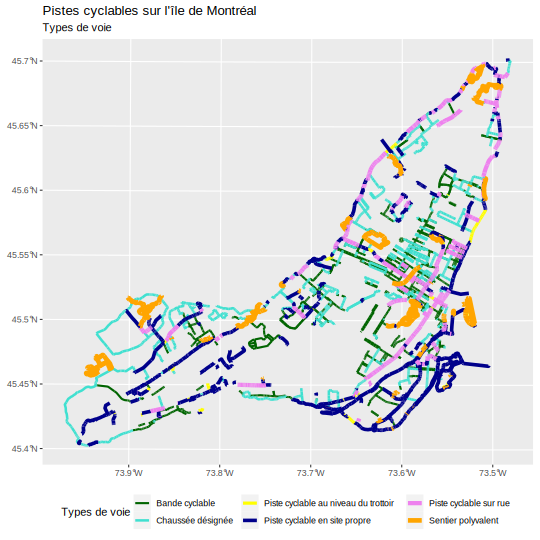
\includegraphics[width=540px]{Cours_SpatialR_files/figure-latex/plot-voie7-1} 

}

\caption{Types de voie cyclable sur l'île de Montréal (couleur et taille des traits)}\label{fig:plot-voie7}
\end{figure}

La légende tient compte à la fois de la couleur, et de la taille des traits. De plus, nous l'avons affichée au bas de la figure.

\hypertarget{visualiser-plusieurs-shapefiles}{%
\subsubsection*{\texorpdfstring{Visualiser plusieurs \emph{shapefiles}}{Visualiser plusieurs shapefiles}}\label{visualiser-plusieurs-shapefiles}}


Nous allons maintenant représenter les données vectorielles \texttt{limites\ terrestres}, \texttt{pistes\_cyclables} et \texttt{accidents\_velo} au sein d'une même figure. Il s'agit d'utiliser la fonction \texttt{geom\_sf} pour chaque couche de données et de les combiner en utilisant le \texttt{+}.

\begin{Shaded}
\begin{Highlighting}[]
\KeywordTok{ggplot}\NormalTok{()}\OperatorTok{+}
\StringTok{  }\KeywordTok{geom_sf}\NormalTok{(}\DataTypeTok{data =}\NormalTok{ limites_terrestres, }\DataTypeTok{size =} \DecValTok{1}\NormalTok{, }\DataTypeTok{color =} \StringTok{"black"}\NormalTok{, }\DataTypeTok{fill =} \StringTok{"white"}\NormalTok{)}\OperatorTok{+}
\StringTok{  }\KeywordTok{geom_sf}\NormalTok{(}\DataTypeTok{data =}\NormalTok{ pistes_cyclables, }\DataTypeTok{size =} \DecValTok{1}\NormalTok{, }\DataTypeTok{color =} \StringTok{"darkgreen"}\NormalTok{)}\OperatorTok{+}
\StringTok{  }\KeywordTok{geom_sf}\NormalTok{(}\DataTypeTok{data =}\NormalTok{ accidents_velo, }\DataTypeTok{pch =} \DecValTok{19}\NormalTok{, }\DataTypeTok{cex =} \FloatTok{1.25}\NormalTok{, }\DataTypeTok{color =} \StringTok{"red"}\NormalTok{)}\OperatorTok{+}
\StringTok{  }\KeywordTok{ggtitle}\NormalTok{(}\StringTok{"Pistes cyclables sur l'île de Montréal et Accidents routiers impliquant des vélos"}\NormalTok{)}
\end{Highlighting}
\end{Shaded}

\begin{figure}

{\centering \includegraphics[width=540px]{Cours_SpatialR_files/figure-latex/plot-all1-1} 

}

\caption{Pistes cyclables et position des accidents routiers impliquant des bicyclettes sur l'île de Montréal}\label{fig:plot-all1}
\end{figure}

Nous pouvons créer une carte plus précise qui spécifie les types de voie cyclable et ajouter une légende.

\begin{Shaded}
\begin{Highlighting}[]
\KeywordTok{ggplot}\NormalTok{()}\OperatorTok{+}
\StringTok{  }\KeywordTok{geom_sf}\NormalTok{(}\DataTypeTok{data =}\NormalTok{ limites_terrestres, }\DataTypeTok{size =} \DecValTok{1}\NormalTok{, }\DataTypeTok{color =} \StringTok{"black"}\NormalTok{, }\DataTypeTok{fill =} \StringTok{"white"}\NormalTok{)}\OperatorTok{+}
\StringTok{  }\KeywordTok{geom_sf}\NormalTok{(}\DataTypeTok{data =}\NormalTok{ pistes_cyclables, }\DataTypeTok{size =} \FloatTok{1.5}\NormalTok{, }\KeywordTok{aes}\NormalTok{(}\DataTypeTok{color =}\NormalTok{ TYPE_VOIE),  }\DataTypeTok{show.legend =} \StringTok{"line"}\NormalTok{)}\OperatorTok{+}
\StringTok{  }\KeywordTok{scale_color_manual}\NormalTok{(}\DataTypeTok{values =}\NormalTok{ couleurs_voie,}\DataTypeTok{name =} \StringTok{"Types de voie"}\NormalTok{)}\OperatorTok{+}
\StringTok{  }\KeywordTok{geom_sf}\NormalTok{(}\DataTypeTok{data =}\NormalTok{ accidents_velo, }\DataTypeTok{pch =} \DecValTok{24}\NormalTok{, }\DataTypeTok{cex =} \DecValTok{2}\NormalTok{, }\DataTypeTok{fill =} \StringTok{"red"}\NormalTok{, }\DataTypeTok{color =} \StringTok{"black"}\NormalTok{)}\OperatorTok{+}
\StringTok{  }\KeywordTok{ggtitle}\NormalTok{(}\StringTok{"Types de voie cyclable et Accidents routiers impliquant des vélos"}\NormalTok{)}\OperatorTok{+}
\KeywordTok{theme}\NormalTok{(}
      \CommentTok{#Caractéristiques de la figure elle-même}
      \DataTypeTok{panel.background =} \KeywordTok{element_rect}\NormalTok{(}\DataTypeTok{fill =} \StringTok{"black"}\NormalTok{), }\CommentTok{#le dessous de la carte}
      \DataTypeTok{plot.background =} \KeywordTok{element_rect}\NormalTok{(}\DataTypeTok{fill =} \StringTok{"black"}\NormalTok{),  }\CommentTok{#le contour de la carte}
      \DataTypeTok{panel.grid.major =} \KeywordTok{element_blank}\NormalTok{(),              }\CommentTok{#retirer la grille cartésienne}
      \DataTypeTok{axis.ticks =} \KeywordTok{element_blank}\NormalTok{(),                    }\CommentTok{#retirer les traits sur les axes}
      \DataTypeTok{axis.text.x =} \KeywordTok{element_blank}\NormalTok{(),                   }\CommentTok{#retirer les traits les noms ou les numéros de ces traits}
      \DataTypeTok{axis.text.y =} \KeywordTok{element_blank}\NormalTok{(),}
      \DataTypeTok{plot.title =} \KeywordTok{element_text}\NormalTok{(}\DataTypeTok{colour =} \StringTok{"white"}\NormalTok{, }\DataTypeTok{size =} \DecValTok{16}\NormalTok{, }\DataTypeTok{hjust =} \FloatTok{0.5}\NormalTok{), }\CommentTok{#Centrer le titre de la carte}
      \CommentTok{#Caractéristiques de la légende}
      \DataTypeTok{legend.position =} \StringTok{"top"}\NormalTok{,                         }\CommentTok{#position de la légende}
      \DataTypeTok{legend.title =} \KeywordTok{element_text}\NormalTok{(}\DataTypeTok{colour=}\StringTok{"blue"}\NormalTok{, }\DataTypeTok{size =} \DecValTok{11}\NormalTok{, }\DataTypeTok{face =} \StringTok{"bold"}\NormalTok{), }\CommentTok{#titre de la légende}
      \DataTypeTok{legend.text =} \KeywordTok{element_text}\NormalTok{(}\DataTypeTok{size =} \DecValTok{10}\NormalTok{, }\DataTypeTok{face =} \StringTok{"italic"}\NormalTok{),               }\CommentTok{#texte des éléments de la légende}
      \DataTypeTok{legend.background =} \KeywordTok{element_rect}\NormalTok{(}\DataTypeTok{fill =} \StringTok{"white"}\NormalTok{, }\DataTypeTok{size =} \DecValTok{1}\NormalTok{, }\DataTypeTok{linetype =} \StringTok{"solid"}\NormalTok{, }\DataTypeTok{colour =} \StringTok{"red"}\NormalTok{), }\CommentTok{#rectangle autour de la légende}
      \DataTypeTok{legend.key =} \KeywordTok{element_rect}\NormalTok{(}\DataTypeTok{fill =} \StringTok{"white"}\NormalTok{)        }\CommentTok{#couleur blanche sous les éléments de la légende}
\NormalTok{)}
\end{Highlighting}
\end{Shaded}

\begin{figure}

{\centering \includegraphics[width=540px]{Cours_SpatialR_files/figure-latex/plot-all2-1} 

}

\caption{Types de voie cyclable et position des accidents routiers impliquant des bicyclettes sur l'île de Montréal.}\label{fig:plot-all2}
\end{figure}

La fonction \texttt{theme()} permet d'ajuster l'apparence de la carte (couleur du fond, couleur, taille et position du titre, format de la légende, etc.). Le chapitre \href{https://ggplot2.tidyverse.org/reference/theme.html}{Modify components of theme} \citep{Wickham_ggplot2_2016} énumère l'ensemble des paramètres pouvant être modifiés pour changer l'apparence d'une carte.

\hypertarget{reprojection-de-donnuxe9es-vectorielles-sous-r}{%
\subsection{Reprojection de données vectorielles sous R}\label{reprojection-de-donnuxe9es-vectorielles-sous-r}}

Dans cette section vous apprendrez à manipuler le système de coordonnées de référence de données vectorielles. Nous avons vu en début de leçon que les données utilisées sont dans la projection de Mercator transverse (\texttt{tmerc}) et utilisent le Système de référence géodésique nord-américan de 1983 (\texttt{NAD83}). Par exemple, pour connaître le SCR des données \texttt{limites\_terrestres}, nous avions fait:

\begin{Shaded}
\begin{Highlighting}[]
\KeywordTok{st_crs}\NormalTok{(limites_terrestres)}
\end{Highlighting}
\end{Shaded}

\begin{verbatim}
Coordinate Reference System:
  User input: 32188 
  wkt:
PROJCS["NAD83 / MTM zone 8",
    GEOGCS["NAD83",
        DATUM["North_American_Datum_1983",
            SPHEROID["GRS 1980",6378137,298.257222101,
                AUTHORITY["EPSG","7019"]],
            TOWGS84[0,0,0,0,0,0,0],
            AUTHORITY["EPSG","6269"]],
        PRIMEM["Greenwich",0,
            AUTHORITY["EPSG","8901"]],
        UNIT["degree",0.0174532925199433,
            AUTHORITY["EPSG","9122"]],
        AUTHORITY["EPSG","4269"]],
    PROJECTION["Transverse_Mercator"],
    PARAMETER["latitude_of_origin",0],
    PARAMETER["central_meridian",-73.5],
    PARAMETER["scale_factor",0.9999],
    PARAMETER["false_easting",304800],
    PARAMETER["false_northing",0],
    UNIT["metre",1,
        AUTHORITY["EPSG","9001"]],
    AXIS["E(X)",EAST],
    AXIS["N(Y)",NORTH],
    AUTHORITY["EPSG","32188"]]
\end{verbatim}

Nous allons maintenant transformer le SCR vers la projection de Robinson (\texttt{robin}) et le Système géodésique mondial de 1984 (\texttt{WGS84}). Pour se faire nous utilisons la fonction \texttt{st\_transform} de la librarie \texttt{st}.

\begin{Shaded}
\begin{Highlighting}[]
\NormalTok{limites_terrestres_rob <-}\StringTok{ }\KeywordTok{st_transform}\NormalTok{(limites_terrestres,}
    \KeywordTok{CRS}\NormalTok{(}\StringTok{"+proj=robin +datum=WGS84"}\NormalTok{))}
\end{Highlighting}
\end{Shaded}

Comparons les données transformées avec les données initiales. Pour se faire, nous voulons représenter les deux cartes une au-dessous de l'autre. La librarie \texttt{ggpubr} permet de créer facilement des figures avec des panneaux multiples. Installez la librarie si ce n'est pas déjà fait, et chargez-là dans votre session de travail.

\begin{Shaded}
\begin{Highlighting}[]
\KeywordTok{library}\NormalTok{(ggpubr)}
\end{Highlighting}
\end{Shaded}

\begin{Shaded}
\begin{Highlighting}[]
\NormalTok{carte1<-}\KeywordTok{ggplot}\NormalTok{()}\OperatorTok{+}
\StringTok{  }\KeywordTok{geom_sf}\NormalTok{(}\DataTypeTok{data =}\NormalTok{ limites_terrestres, }\DataTypeTok{size =} \DecValTok{1}\NormalTok{, }\DataTypeTok{color =} \StringTok{"black"}\NormalTok{, }\DataTypeTok{fill =} \StringTok{"white"}\NormalTok{) }\OperatorTok{+}
\StringTok{  }\KeywordTok{ggtitle}\NormalTok{(}\StringTok{"Projection Mercator"}\NormalTok{)}
\NormalTok{carte2<-}\KeywordTok{ggplot}\NormalTok{()}\OperatorTok{+}
\StringTok{  }\KeywordTok{geom_sf}\NormalTok{(}\DataTypeTok{data =}\NormalTok{ limites_terrestres_rob, }\DataTypeTok{size =} \DecValTok{1}\NormalTok{, }\DataTypeTok{color =} \StringTok{"black"}\NormalTok{, }\DataTypeTok{fill =} \StringTok{"yellow"}\NormalTok{) }\OperatorTok{+}
\StringTok{  }\KeywordTok{ggtitle}\NormalTok{(}\StringTok{"Projection Robinson"}\NormalTok{)}
\NormalTok{figure <-}\StringTok{ }\KeywordTok{ggarrange}\NormalTok{(carte1, carte2, }\DataTypeTok{labels =} \KeywordTok{c}\NormalTok{(}\StringTok{"A"}\NormalTok{,}\StringTok{"B"}\NormalTok{),}\DataTypeTok{ncol =} \DecValTok{1}\NormalTok{, }\DataTypeTok{nrow =} \DecValTok{2}\NormalTok{)}
\NormalTok{figure}
\end{Highlighting}
\end{Shaded}

\begin{figure}

{\centering 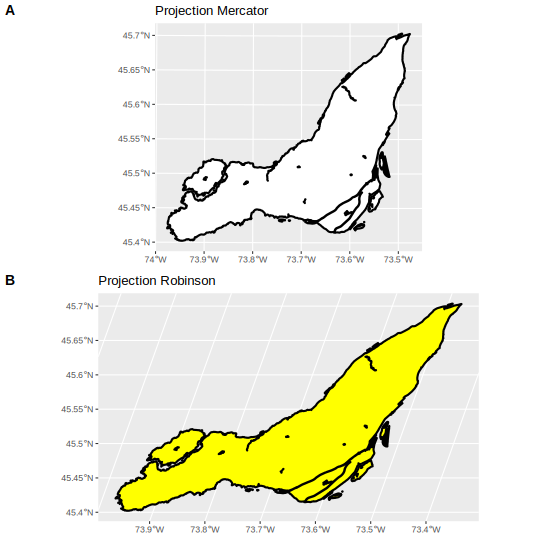
\includegraphics[width=540px]{Cours_SpatialR_files/figure-latex/plot-terre2-1} 

}

\caption{Limites terrestres de l'île de Montréal selon les projections Mercartor (A) et Robinson (B)}\label{fig:plot-terre2}
\end{figure}

Finalement, pour sauvegarder des données vectorielles, nous utilisons la fonction \texttt{st\_write} de la librarie \texttt{st}, de la même façon que nous avons utilisé la fonction \texttt{st\_read} en début de leçon. Par exemple, sauvons les données \texttt{limites\_terrestres\_rob} que nous venons de créer.

\begin{Shaded}
\begin{Highlighting}[]
\NormalTok{chemin<-}\StringTok{"D:/votrechemin/SCI1031/Module3/Donnees/"}
\NormalTok{nom_du_fichier<-}\StringTok{ }\KeywordTok{paste}\NormalTok{(chemin, }\StringTok{"/Montreal_Velo/terre/terre_rob_shp.shp"}\NormalTok{, }\DataTypeTok{sep =} \StringTok{""}\NormalTok{)}
\KeywordTok{st_read}\NormalTok{(limites_terrestres_rob,nom_du_fichier)}
\end{Highlighting}
\end{Shaded}

\hypertarget{exercice-2}{%
\section{Exercice}\label{exercice-2}}

\hypertarget{mat}{%
\chapter{Les données matricielles}\label{mat}}

L'objectif principal de ce module est

À la fin de ce module vous saurez:

\begin{itemize}
\item
\item
\item
\end{itemize}

Vous utiliserez les librairies suivantes:

\begin{itemize}
\item
\item
\end{itemize}

Vous apprendrez à utiliser les fonctions suivantes:

\begin{itemize}
\item
\item
\end{itemize}

Dans la section Leçon, vous utiliserez des données XYXYX

Dans la section Exercice, vous utiliserez XXXXX

\hypertarget{leuxe7on-3}{%
\section{Leçon}\label{leuxe7on-3}}

\hypertarget{introduction-aux-donnuxe9es-matricielles-sous-r}{%
\subsection{Introduction aux données matricielles sous R}\label{introduction-aux-donnuxe9es-matricielles-sous-r}}

\begin{itemize}
\tightlist
\item
  Lire et explorer les attributs d'un raster
\item
  Comprendre le SCR
\item
  Gérer les données manquantes et les mauvaises données
\item
  Raster mono-bande et multi-bande
\item
  Écrire des données matricielles
\end{itemize}

\hypertarget{visualisation-de-rasters-sous-r}{%
\subsection{Visualisation de rasters sous R}\label{visualisation-de-rasters-sous-r}}

\begin{itemize}
\tightlist
\item
  Utiliser ggplot pour visualiser les rasters
\item
  Visualiser plusieurs couches matricielles
\item
  Visualiser des données matricielles et vectorielles au sein d'une même figure
\end{itemize}

\hypertarget{reprojection-de-donnuxe9es-matricielles-sous-r}{%
\subsection{Reprojection de données matricielles sous R}\label{reprojection-de-donnuxe9es-matricielles-sous-r}}

\begin{itemize}
\tightlist
\item
  Manipuler le SCR
\item
  Manipuler la résolution
\end{itemize}

\hypertarget{manipulation-de-rasters-multi-bande-sous-r}{%
\subsection{Manipulation de rasters multi-bande sous R}\label{manipulation-de-rasters-multi-bande-sous-r}}

\begin{itemize}
\tightlist
\item
  Visualiser des rasters multi-bande
\item
  Manipuler des objets RasterStack
\item
  Manipuler des objets RasterBrick
\end{itemize}

\hypertarget{exercice-3}{%
\section{Exercice}\label{exercice-3}}

\hypertarget{carto}{%
\chapter{La cartographie}\label{carto}}

L'objectif principal de ce module est

À la fin de ce module vous saurez:

\begin{itemize}
\item
\item
\item
\end{itemize}

Vous utiliserez les librairies suivantes:

\begin{itemize}
\item
\item
\end{itemize}

Vous apprendrez à utiliser les fonctions suivantes:

\begin{itemize}
\item
\item
\end{itemize}

Dans la section Leçon, vous utiliserez des données XYXYX

Dans la section Exercice, vous utiliserez XXXXX

\hypertarget{leuxe7on-4}{%
\section{Leçon}\label{leuxe7on-4}}

\hypertarget{cartographie-dobjets-vectoriels}{%
\subsection{Cartographie d'objets vectoriels}\label{cartographie-dobjets-vectoriels}}

\begin{itemize}
\tightlist
\item
  Carte de base (graticules, échelle, rose des vents, légende, titre).
\end{itemize}

\hypertarget{cartographie-dobjets-matriciels}{%
\subsection{Cartographie d'objets matriciels}\label{cartographie-dobjets-matriciels}}

\begin{itemize}
\tightlist
\item
  Carte de base, rampe de couleurs.
\end{itemize}

\hypertarget{cartographie-en-ligne}{%
\subsection{Cartographie en ligne}\label{cartographie-en-ligne}}

\begin{itemize}
\tightlist
\item
  GoogleMap
\item
  Leaflet
\item
  OpenStreetMap
\end{itemize}

\hypertarget{exercice-4}{%
\section{Exercice}\label{exercice-4}}

\hypertarget{map_vec}{%
\chapter{La manipulation de données vectorielles}\label{map_vec}}

L'objectif principal de ce module est

À la fin de ce module vous saurez:

\begin{itemize}
\item
\item
\item
\end{itemize}

Vous utiliserez les librairies suivantes:

\begin{itemize}
\item
\item
\end{itemize}

Vous apprendrez à utiliser les fonctions suivantes:

\begin{itemize}
\item
\item
\end{itemize}

Dans la section Leçon, vous utiliserez des données XYXYX

Dans la section Exercice, vous utiliserez XXXXX

\hypertarget{leuxe7on-5}{%
\section{Leçon}\label{leuxe7on-5}}

\hypertarget{opuxe9rations-de-base}{%
\subsection{Opérations de base}\label{opuxe9rations-de-base}}

\begin{itemize}
\tightlist
\item
  Supprimer des champs, ajouter des champs, modifier des valeurs de champs, trier la table des attributs.
\end{itemize}

\hypertarget{opuxe9ration-sur-une-couche-vectorielle}{%
\subsection{Opération sur une couche vectorielle}\label{opuxe9ration-sur-une-couche-vectorielle}}

\begin{itemize}
\tightlist
\item
  Jointure par identifiant, suppression de données, extraction par attributs, dissolution de polygones.
\end{itemize}

\hypertarget{opuxe9ration-sur-plusieurs-couches-vectorielles}{%
\subsection{Opération sur plusieurs couches vectorielles}\label{opuxe9ration-sur-plusieurs-couches-vectorielles}}

\begin{itemize}
\tightlist
\item
  Combinaison de couches, jointure spatiale, intersection de couches, découpage d'une couche.
\end{itemize}

\hypertarget{exercice-5}{%
\section{Exercice}\label{exercice-5}}

\hypertarget{map_mat}{%
\chapter{La manipulation de données matricielles}\label{map_mat}}

L'objectif principal de ce module est

À la fin de ce module vous saurez:

\begin{itemize}
\item
\item
\item
\end{itemize}

Vous utiliserez les librairies suivantes:

\begin{itemize}
\item
\item
\end{itemize}

Vous apprendrez à utiliser les fonctions suivantes:

\begin{itemize}
\item
\item
\end{itemize}

Dans la section Leçon, vous utiliserez des données XYXYX

Dans la section Exercice, vous utiliserez XXXXX

\hypertarget{leuxe7on-6}{%
\section{Leçon}\label{leuxe7on-6}}

\hypertarget{opuxe9rations-de-base-1}{%
\subsection{Opérations de base}\label{opuxe9rations-de-base-1}}

\begin{itemize}
\tightlist
\item
  Création d'un raster, création d'un raster multi-couches, opérations mathématiques et statistiques élémentaires.
\end{itemize}

\hypertarget{opuxe9ration-sur-un-raster}{%
\subsection{Opération sur un raster}\label{opuxe9ration-sur-un-raster}}

\begin{itemize}
\tightlist
\item
  Extraction d'un sous-ensemble de données, suppression de données, modification de données, changement de position
\end{itemize}

\hypertarget{opuxe9ration-sur-plusieurs-rasters}{%
\subsection{Opération sur plusieurs rasters}\label{opuxe9ration-sur-plusieurs-rasters}}

\begin{itemize}
\tightlist
\item
  Combinaison de rasters, jointure spatiale, intersection de couches, découpage d'une couche.
\end{itemize}

\hypertarget{exercice-6}{%
\section{Exercice}\label{exercice-6}}

\hypertarget{spatiotemp}{%
\chapter{Les données spatiotemporelles}\label{spatiotemp}}

L'objectif principal de ce module est

À la fin de ce module vous saurez:

\begin{itemize}
\item
\item
\item
\end{itemize}

Vous utiliserez les librairies suivantes:

\begin{itemize}
\item
\item
\end{itemize}

Vous apprendrez à utiliser les fonctions suivantes:

\begin{itemize}
\item
\item
\end{itemize}

Dans la section Leçon, vous utiliserez des données XYXYX

Dans la section Exercice, vous utiliserez XXXXX

\hypertarget{leuxe7on-7}{%
\section{Leçon}\label{leuxe7on-7}}

\hypertarget{propriuxe9tuxe9s-des-donnuxe9es-spatiotemporelles}{%
\subsection{Propriétés des données spatiotemporelles}\label{propriuxe9tuxe9s-des-donnuxe9es-spatiotemporelles}}

\hypertarget{introduction-uxe0-la-librairie-r-spacetime}{%
\subsection{Introduction à la librairie R spacetime}\label{introduction-uxe0-la-librairie-r-spacetime}}

\begin{itemize}
\tightlist
\item
  Classes de données spatiotemporelles
\item
  Création d'objet ST
\item
  Manipulation de bases de données spatiotemporelles
\end{itemize}

\hypertarget{visualisation}{%
\subsection{Visualisation}\label{visualisation}}

\begin{itemize}
\tightlist
\item
  Figure à panneaux multiples
\item
  Figure espace-temps
\item
  Figure animée
\end{itemize}

\hypertarget{exercice-7}{%
\section{Exercice}\label{exercice-7}}

\hypertarget{analyse}{%
\chapter{L'analyse de données spatiales}\label{analyse}}

L'objectif principal de ce module est

À la fin de ce module vous saurez:

\begin{itemize}
\item
\item
\item
\end{itemize}

Vous utiliserez les librairies suivantes:

\begin{itemize}
\item
\item
\end{itemize}

Vous apprendrez à utiliser les fonctions suivantes:

\begin{itemize}
\item
\item
\end{itemize}

Dans la section Leçon, vous utiliserez des données XYXYX

Dans la section Exercice, vous utiliserez XXXXX

\hypertarget{leuxe7on-8}{%
\section{Leçon}\label{leuxe7on-8}}

\hypertarget{distance}{%
\subsection{Distance}\label{distance}}

\begin{itemize}
\tightlist
\item
  Distance entre des points, distance entre des cellules, matrice de distance, distance pour les coordonnées angulaires.
\end{itemize}

\hypertarget{configuration-spatiale}{%
\subsection{Configuration spatiale}\label{configuration-spatiale}}

\begin{itemize}
\tightlist
\item
  Proximité, plus proche voisin, frontière, superficie, connectivité, inclusion, zones tampons, matrice de résistance.
\end{itemize}

\hypertarget{autocorruxe9lation-spatiale}{%
\subsection{Autocorrélation spatiale}\label{autocorruxe9lation-spatiale}}

\begin{itemize}
\tightlist
\item
  Covariance et correlation, autocorrelation temporelle et spatiale, indice de Moran.
\end{itemize}

\hypertarget{exercice-8}{%
\section{Exercice}\label{exercice-8}}

  \bibliography{refs.bib}

\printindex

\end{document}
